\documentclass[]{krantz}
\usepackage{lmodern}
\usepackage{amssymb,amsmath}
\usepackage{ifxetex,ifluatex}
\usepackage{fixltx2e} % provides \textsubscript
\ifnum 0\ifxetex 1\fi\ifluatex 1\fi=0 % if pdftex
  \usepackage[T1]{fontenc}
  \usepackage[utf8]{inputenc}
\else % if luatex or xelatex
  \ifxetex
    \usepackage{mathspec}
  \else
    \usepackage{fontspec}
  \fi
  \defaultfontfeatures{Ligatures=TeX,Scale=MatchLowercase}
\fi
% use upquote if available, for straight quotes in verbatim environments
\IfFileExists{upquote.sty}{\usepackage{upquote}}{}
% use microtype if available
\IfFileExists{microtype.sty}{%
\usepackage[]{microtype}
\UseMicrotypeSet[protrusion]{basicmath} % disable protrusion for tt fonts
}{}
\PassOptionsToPackage{hyphens}{url} % url is loaded by hyperref
\usepackage[unicode=true]{hyperref}
\PassOptionsToPackage{usenames,dvipsnames}{color} % color is loaded by hyperref
\hypersetup{
            pdftitle={Reproducible Finance with R},
            pdfauthor={Jonathan K. Regenstein, Jr.},
            colorlinks=true,
            linkcolor=Maroon,
            citecolor=Blue,
            urlcolor=Blue,
            breaklinks=true}
\urlstyle{same}  % don't use monospace font for urls
\usepackage{natbib}
\bibliographystyle{apalike}
\usepackage{color}
\usepackage{fancyvrb}
\newcommand{\VerbBar}{|}
\newcommand{\VERB}{\Verb[commandchars=\\\{\}]}
\DefineVerbatimEnvironment{Highlighting}{Verbatim}{commandchars=\\\{\}}
% Add ',fontsize=\small' for more characters per line
\usepackage{framed}
\definecolor{shadecolor}{RGB}{248,248,248}
\newenvironment{Shaded}{\begin{snugshade}}{\end{snugshade}}
\newcommand{\KeywordTok}[1]{\textcolor[rgb]{0.13,0.29,0.53}{\textbf{#1}}}
\newcommand{\DataTypeTok}[1]{\textcolor[rgb]{0.13,0.29,0.53}{#1}}
\newcommand{\DecValTok}[1]{\textcolor[rgb]{0.00,0.00,0.81}{#1}}
\newcommand{\BaseNTok}[1]{\textcolor[rgb]{0.00,0.00,0.81}{#1}}
\newcommand{\FloatTok}[1]{\textcolor[rgb]{0.00,0.00,0.81}{#1}}
\newcommand{\ConstantTok}[1]{\textcolor[rgb]{0.00,0.00,0.00}{#1}}
\newcommand{\CharTok}[1]{\textcolor[rgb]{0.31,0.60,0.02}{#1}}
\newcommand{\SpecialCharTok}[1]{\textcolor[rgb]{0.00,0.00,0.00}{#1}}
\newcommand{\StringTok}[1]{\textcolor[rgb]{0.31,0.60,0.02}{#1}}
\newcommand{\VerbatimStringTok}[1]{\textcolor[rgb]{0.31,0.60,0.02}{#1}}
\newcommand{\SpecialStringTok}[1]{\textcolor[rgb]{0.31,0.60,0.02}{#1}}
\newcommand{\ImportTok}[1]{#1}
\newcommand{\CommentTok}[1]{\textcolor[rgb]{0.56,0.35,0.01}{\textit{#1}}}
\newcommand{\DocumentationTok}[1]{\textcolor[rgb]{0.56,0.35,0.01}{\textbf{\textit{#1}}}}
\newcommand{\AnnotationTok}[1]{\textcolor[rgb]{0.56,0.35,0.01}{\textbf{\textit{#1}}}}
\newcommand{\CommentVarTok}[1]{\textcolor[rgb]{0.56,0.35,0.01}{\textbf{\textit{#1}}}}
\newcommand{\OtherTok}[1]{\textcolor[rgb]{0.56,0.35,0.01}{#1}}
\newcommand{\FunctionTok}[1]{\textcolor[rgb]{0.00,0.00,0.00}{#1}}
\newcommand{\VariableTok}[1]{\textcolor[rgb]{0.00,0.00,0.00}{#1}}
\newcommand{\ControlFlowTok}[1]{\textcolor[rgb]{0.13,0.29,0.53}{\textbf{#1}}}
\newcommand{\OperatorTok}[1]{\textcolor[rgb]{0.81,0.36,0.00}{\textbf{#1}}}
\newcommand{\BuiltInTok}[1]{#1}
\newcommand{\ExtensionTok}[1]{#1}
\newcommand{\PreprocessorTok}[1]{\textcolor[rgb]{0.56,0.35,0.01}{\textit{#1}}}
\newcommand{\AttributeTok}[1]{\textcolor[rgb]{0.77,0.63,0.00}{#1}}
\newcommand{\RegionMarkerTok}[1]{#1}
\newcommand{\InformationTok}[1]{\textcolor[rgb]{0.56,0.35,0.01}{\textbf{\textit{#1}}}}
\newcommand{\WarningTok}[1]{\textcolor[rgb]{0.56,0.35,0.01}{\textbf{\textit{#1}}}}
\newcommand{\AlertTok}[1]{\textcolor[rgb]{0.94,0.16,0.16}{#1}}
\newcommand{\ErrorTok}[1]{\textcolor[rgb]{0.64,0.00,0.00}{\textbf{#1}}}
\newcommand{\NormalTok}[1]{#1}
\usepackage{longtable,booktabs}
% Fix footnotes in tables (requires footnote package)
\IfFileExists{footnote.sty}{\usepackage{footnote}\makesavenoteenv{long table}}{}
\usepackage{graphicx,grffile}
\makeatletter
\def\maxwidth{\ifdim\Gin@nat@width>\linewidth\linewidth\else\Gin@nat@width\fi}
\def\maxheight{\ifdim\Gin@nat@height>\textheight\textheight\else\Gin@nat@height\fi}
\makeatother
% Scale images if necessary, so that they will not overflow the page
% margins by default, and it is still possible to overwrite the defaults
% using explicit options in \includegraphics[width, height, ...]{}
\setkeys{Gin}{width=\maxwidth,height=\maxheight,keepaspectratio}
\IfFileExists{parskip.sty}{%
\usepackage{parskip}
}{% else
\setlength{\parindent}{0pt}
\setlength{\parskip}{6pt plus 2pt minus 1pt}
}
\setlength{\emergencystretch}{3em}  % prevent overfull lines
\providecommand{\tightlist}{%
  \setlength{\itemsep}{0pt}\setlength{\parskip}{0pt}}
\setcounter{secnumdepth}{5}
% Redefines (sub)paragraphs to behave more like sections
\ifx\paragraph\undefined\else
\let\oldparagraph\paragraph
\renewcommand{\paragraph}[1]{\oldparagraph{#1}\mbox{}}
\fi
\ifx\subparagraph\undefined\else
\let\oldsubparagraph\subparagraph
\renewcommand{\subparagraph}[1]{\oldsubparagraph{#1}\mbox{}}
\fi

% set default figure placement to htbp
\makeatletter
\def\fps@figure{htbp}
\makeatother

\usepackage{booktabs}
\usepackage{longtable}
\usepackage[bf,singlelinecheck=off]{caption}

\usepackage{framed,color}
\definecolor{shadecolor}{RGB}{248,248,248}

\renewcommand{\textfraction}{0.05}
\renewcommand{\topfraction}{0.8}
\renewcommand{\bottomfraction}{0.8}
\renewcommand{\floatpagefraction}{0.75}

\renewenvironment{quote}{\begin{VF}}{\end{VF}}
\let\oldhref\href
\renewcommand{\href}[2]{#2\footnote{\url{#1}}}

\makeatletter
\newenvironment{kframe}{%
\medskip{}
\setlength{\fboxsep}{.8em}
 \def\at@end@of@kframe{}%
 \ifinner\ifhmode%
  \def\at@end@of@kframe{\end{minipage}}%
  \begin{minipage}{\columnwidth}%
 \fi\fi%
 \def\FrameCommand##1{\hskip\@totalleftmargin \hskip-\fboxsep
 \colorbox{shadecolor}{##1}\hskip-\fboxsep
     % There is no \\@totalrightmargin, so:
     \hskip-\linewidth \hskip-\@totalleftmargin \hskip\columnwidth}%
 \MakeFramed {\advance\hsize-\width
   \@totalleftmargin\z@ \linewidth\hsize
   \@setminipage}}%
 {\par\unskip\endMakeFramed%
 \at@end@of@kframe}
\makeatother

\renewenvironment{Shaded}{\begin{kframe}}{\end{kframe}}

\usepackage{makeidx}
\makeindex

\urlstyle{tt}

\usepackage{amsthm}
\makeatletter
\def\thm@space@setup{%
  \thm@preskip=8pt plus 2pt minus 4pt
  \thm@postskip=\thm@preskip
}
\makeatother

\frontmatter

\title{Reproducible Finance with R}
\author{Jonathan K. Regenstein, Jr.}
\date{2018-01-17}

\let\BeginKnitrBlock\begin \let\EndKnitrBlock\end
\begin{document}
\maketitle

% you may need to leave a few empty pages before the dedication page

%\cleardoublepage\newpage\thispagestyle{empty}\null
%\cleardoublepage\newpage\thispagestyle{empty}\null
%\cleardoublepage\newpage
\thispagestyle{empty}

\begin{center}
To my son,

without whom I should have finished this book two years earlier
%\includegraphics{images/dedication.pdf}
\end{center}

\setlength{\abovedisplayskip}{-5pt}
\setlength{\abovedisplayshortskip}{-5pt}

{
\hypersetup{linkcolor=black}
\setcounter{tocdepth}{0}
\tableofcontents
}
\listoftables
\listoffigures
\chapter*{Preface}\label{preface}


Hi there, this is my great book.

\section*{Why read this book}\label{why-read-this-book}


It is very important\ldots{}

\section*{Structure of the book}\label{structure-of-the-book}


Chapter \ref{prices-to-returns} introduces prices to returns \ldots{}

\section*{About the Author}\label{about-the-author}


Jonathan Regenstein is the Director of Financial Services practice at
RStudio.

\section*{Software information and
conventions}\label{software-information-and-conventions}


I used the \textbf{knitr}\index{knitr} package \citep{xie2015} and the
\textbf{bookdown}\index{bookdown} package \citep{R-bookdown} to compile
my book. My R session information is shown below:

\begin{Shaded}
\begin{Highlighting}[]
\KeywordTok{sessionInfo}\NormalTok{()}
\end{Highlighting}
\end{Shaded}

\begin{verbatim}
## R version 3.4.0 (2017-04-21)
## Platform: x86_64-pc-linux-gnu (64-bit)
## Running under: Ubuntu 14.04.5 LTS
## 
## Matrix products: default
## BLAS: /usr/lib/openblas-base/libopenblas.so.0
## LAPACK: /usr/lib/lapack/liblapack.so.3.0
## 
## locale:
##  [1] LC_CTYPE=en_US.UTF-8      
##  [2] LC_NUMERIC=C              
##  [3] LC_TIME=en_US.UTF-8       
##  [4] LC_COLLATE=en_US.UTF-8    
##  [5] LC_MONETARY=en_US.UTF-8   
##  [6] LC_MESSAGES=en_US.UTF-8   
##  [7] LC_PAPER=en_US.UTF-8      
##  [8] LC_NAME=C                 
##  [9] LC_ADDRESS=C              
## [10] LC_TELEPHONE=C            
## [11] LC_MEASUREMENT=en_US.UTF-8
## [12] LC_IDENTIFICATION=C       
## 
## attached base packages:
## [1] stats     graphics  grDevices utils     datasets 
## [6] methods   base     
## 
## other attached packages:
##  [1] bindrcpp_0.2                 
##  [2] tibbletime_0.1.0             
##  [3] timetk_0.1.0                 
##  [4] highcharter_0.5.0            
##  [5] tidyquant_0.5.3              
##  [6] quantmod_0.4-11              
##  [7] TTR_0.23-1                   
##  [8] PerformanceAnalytics_1.4.3541
##  [9] xts_0.10-0                   
## [10] zoo_1.8-0                    
## [11] lubridate_1.7.1              
## [12] forcats_0.2.0                
## [13] stringr_1.2.0                
## [14] dplyr_0.7.4                  
## [15] purrr_0.2.4                  
## [16] readr_1.1.1                  
## [17] tidyr_0.7.2                  
## [18] tibble_1.4.1                 
## [19] ggplot2_2.2.1                
## [20] tidyverse_1.2.1              
## 
## loaded via a namespace (and not attached):
##  [1] Rcpp_0.12.13        lattice_0.20-35    
##  [3] utf8_1.1.3          assertthat_0.2.0   
##  [5] rprojroot_1.3-1     digest_0.6.12      
##  [7] psych_1.7.8         R6_2.2.2           
##  [9] cellranger_1.1.0    plyr_1.8.4         
## [11] backports_1.1.2     evaluate_0.10.1    
## [13] blogdown_0.4        httr_1.3.1         
## [15] highr_0.6           pillar_1.0.1       
## [17] rlang_0.1.6         curl_3.1           
## [19] lazyeval_0.2.0      readxl_1.0.0       
## [21] rstudioapi_0.7      data.table_1.10.4-2
## [23] rmarkdown_1.8       labeling_0.3       
## [25] servr_0.8           foreign_0.8-67     
## [27] htmlwidgets_0.9     igraph_1.1.2       
## [29] munsell_0.4.3       broom_0.4.3        
## [31] httpuv_1.3.5        compiler_3.4.0     
## [33] modelr_0.1.1        pkgconfig_2.0.1    
## [35] mnormt_1.5-5        htmltools_0.3.6    
## [37] tidyselect_0.2.3    bookdown_0.5       
## [39] crayon_1.3.4        grid_3.4.0         
## [41] Quandl_2.8.0        nlme_3.1-131       
## [43] jsonlite_1.5        gtable_0.2.0       
## [45] magrittr_1.5        scales_0.4.1       
## [47] rlist_0.4.6.1       cli_1.0.0          
## [49] stringi_1.1.6       reshape2_1.4.2     
## [51] xml2_1.1.1          tools_3.4.0        
## [53] glue_1.1.1          hms_0.4.0          
## [55] rsconnect_0.8.5     parallel_3.4.0     
## [57] yaml_2.1.16         colorspace_1.3-2   
## [59] rvest_0.3.2         knitr_1.18         
## [61] bindr_0.1           haven_1.1.0
\end{verbatim}

Package names are in bold text (e.g., \textbf{rmarkdown}), and inline
code and filenames are formatted in a typewriter font (e.g.,
\texttt{knitr::knit(\textquotesingle{}foo.Rmd\textquotesingle{})}).
Function names are followed by parentheses (e.g.,
\texttt{bookdown::render\_book()}).

\section*{Acknowledgments}\label{acknowledgments}


A lot of people helped me when I was writing the book.

\BeginKnitrBlock{flushright}
Frida Gomam\\
on the Mars
\EndKnitrBlock{flushright}

\mainmatter

\chapter*{Introduction}\label{introduction}


Now unplug your Internet cable, and start doing some serious work.

We have a nice figure in Figure \ref{fig:hello}, and also a table in
Table \ref{tab:iris}.

\begin{Shaded}
\begin{Highlighting}[]
\KeywordTok{par}\NormalTok{(}\DataTypeTok{mar =} \KeywordTok{c}\NormalTok{(}\DecValTok{4}\NormalTok{, }\DecValTok{4}\NormalTok{, }\DecValTok{1}\NormalTok{, .}\DecValTok{1}\NormalTok{))}
\KeywordTok{plot}\NormalTok{(cars, }\DataTypeTok{pch =} \DecValTok{19}\NormalTok{)}
\end{Highlighting}
\end{Shaded}

\begin{figure}
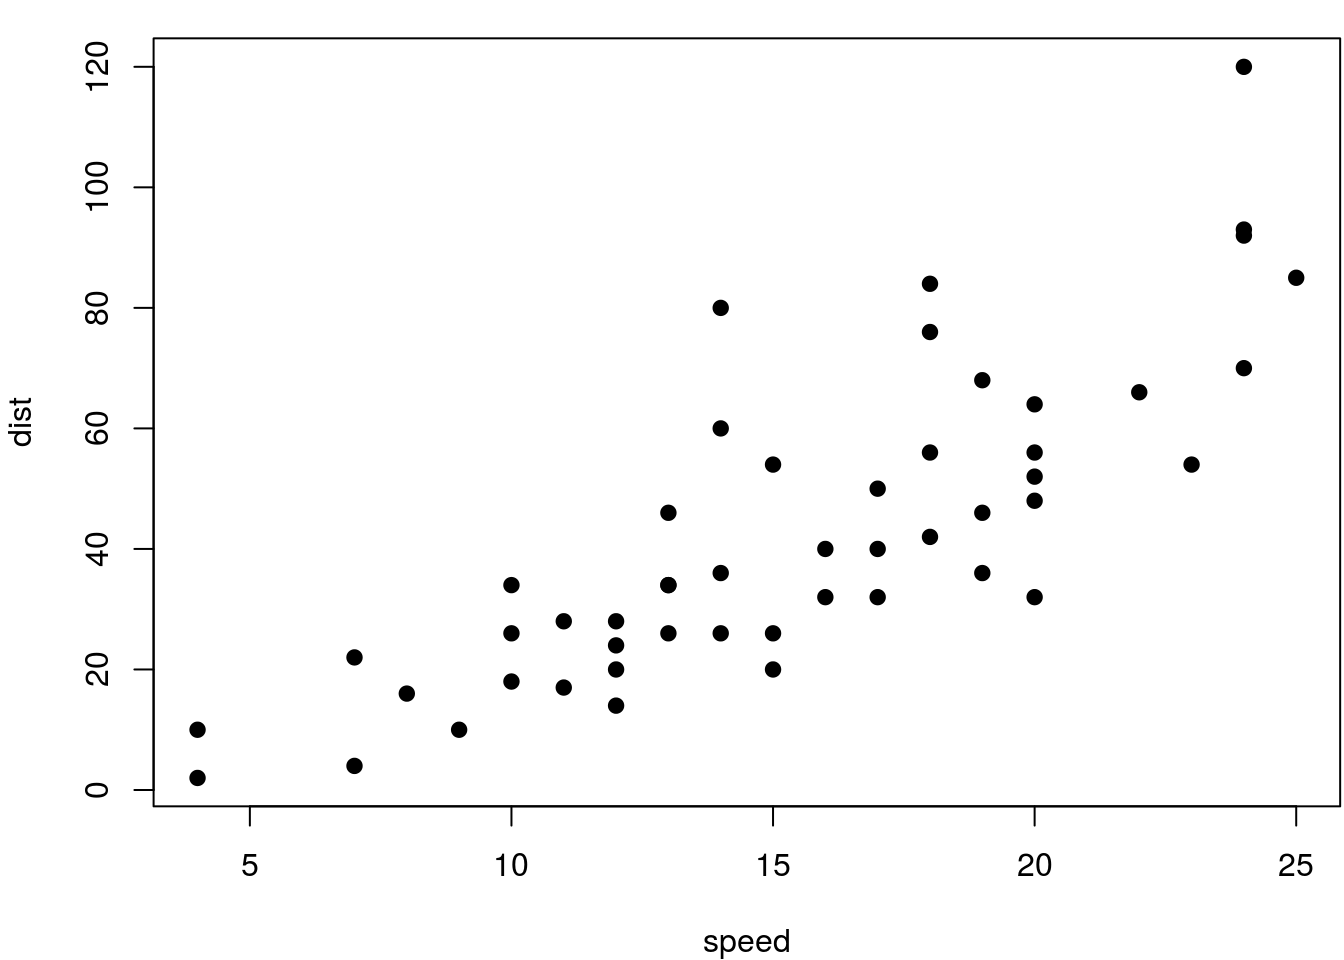
\includegraphics[width=0.9\linewidth]{bookdown_files/figure-latex/hello-1} \caption{Hello World!}\label{fig:hello}
\end{figure}

\begin{Shaded}
\begin{Highlighting}[]
\NormalTok{knitr}\OperatorTok{::}\KeywordTok{kable}\NormalTok{(}
  \KeywordTok{head}\NormalTok{(iris), }\DataTypeTok{caption =} \StringTok{'The boring iris data.'}\NormalTok{,}
  \DataTypeTok{booktabs =} \OtherTok{TRUE}
\NormalTok{)}
\end{Highlighting}
\end{Shaded}

\begin{table}

\caption{\label{tab:iris}The boring iris data.}
\centering
\begin{tabular}[t]{rrrrl}
\toprule
Sepal.Length & Sepal.Width & Petal.Length & Petal.Width & Species\\
\midrule
5.1 & 3.5 & 1.4 & 0.2 & setosa\\
4.9 & 3.0 & 1.4 & 0.2 & setosa\\
4.7 & 3.2 & 1.3 & 0.2 & setosa\\
4.6 & 3.1 & 1.5 & 0.2 & setosa\\
5.0 & 3.6 & 1.4 & 0.2 & setosa\\
5.4 & 3.9 & 1.7 & 0.4 & setosa\\
\bottomrule
\end{tabular}
\end{table}

More chapters to come in \texttt{02-returns.Rmd},
\texttt{03-prices-to-returns}.Rmd, \ldots{}

\chapter*{Returns}\label{returns}


Welcome to our section on asset returns, wherein we will perform the
unglamorous work of taking raw price data for individual assets and
tranforming them into monthly returns for a single portfolio. To map a
data science work flow onto portfolio analysis, those steps encompass
data import, cleaning, wrangling, transformation and initial
visualization. Even though the subtstantive issues are not complex, we
will painstakingly go through the code to ensure that the data
provenance is clear, reproducible and reusable. In fact, we will devote
as much time to this section as we do to any of the sections that are
more analytical. That might seem a bit unbalanced - afterall, quants
don't get paid to import, clean and wrangle data. But it's foundational
to the more complex stuff and when done well, it makes the complex much
less complex.

Furthermore, our partners, collaborators and future selves will thank us
for this effort when they want to update our models or extend our work
or stress test with different assumptions.

Here's what we want to accomplish in this section:

\begin{enumerate}
\def\labelenumi{\arabic{enumi})}
\tightlist
\item
  Import daily prices from the internet.
\item
  Select the adjusted prices only.
\item
  Transform daily prices to monthly prices.
\item
  Transform monthly prices to monthly returns.
\item
  Chart monthly returns.
\item
  Choose allocations or weights for each asset.
\item
  Calculate portfolio monthly returns based on asset monthly returns and
  weights.
\item
  Chart portfolio returns
\item
  Calculate growth of a dollar, given portfolio returns.
\item
  Chart the growth of a dollar
\item
  Save all of our data objects for use by our collaborators and future
  self
\item
  We will use those saved objects throughouth the rest of this book, so
  this work is important!
\end{enumerate}

Our ultimate goal is to constructe a 5-asset portfolio consisting of the
following.

\begin{verbatim}
+ SPY (S&P500 fund) weighted 25%
+ EFA (a non-US equities fund) weighted 25%
+ IJS (a small-cap value fund) weighted 20%
+ EEM (an emerging-markets fund) weighted 20%
+ AGG (a bond fund) weighted 10%
\end{verbatim}

I chose those 5 assets because they seem to offer a balanced blend of
large, small, international, emerging and bond exposure. We will include
several Shiny applications in this book and those will enable you or any
other end user to build a custom portfolio and see how things change.
For the rest of our work inside of this book, we will not change or
deviate from these 5 assets and the chosen portfolio.

That said, changing to different assets and weights does not involve a
heavy lift and I encourage you to experiment with different asset
combinations.

\chapter{Asset Prices to Returns}\label{asset-prices-to-returns}

\subsection*{Importing Asset Prices}\label{importing-asset-prices}


Let's get to step 1 wherein we import adjusted price data for the 5 ETFs
to be used in our porftolio and save them to an \texttt{xts} object
called \texttt{prices}.

First, we need to choose ticker symbols and store them in a vector
called symbols. We do that with
\texttt{symbols\ \textless{}-\ c("SPY","EFA",\ "IJS",\ "EEM","AGG")}.
Those are the tickers for the 5 assets in our portfolio. If you want to
change to different assets for testing, change those tickers.

We will then pass \texttt{symbols} to Yahoo! Finance via the
\texttt{getSymbols()} function from the \texttt{quantmod} package. This
will return an object with the opening price, closing price, adjusted
price, daily high, daily low and daily volume. We don't want to work
with all of those, though. The adjusted price is what we want.

Note that we are enforcing a starting date of ``2013-01-01'' and an end
date of ``2017-12-31''. That means we will be working with 5 years of
data. If you wish to run this script or pull data that is up-to-date as
of today, you can remove the argument \texttt{to\ =\ "2017-12-31"} - but
then your raw data will be different from what is being used in this
book. That's fine, but the numbers will not match after that.

To isolate the adjusted price, we use the \texttt{map()} function from
the \texttt{purrr} package and apply \texttt{Ad(get(.))} to the imported
prices. This will \texttt{get()} the adjusted price from each of our
individual price series. If we wanted the closing price, we would run
\texttt{Cl(get(.))}. That \texttt{.} refers to our initial object. Note
that if you wish to choose different stock tickers, you change the
tickers in the \texttt{symbols} vector.

We could stop here and have the right substance - daily prices for 5
tickers - but the format wouldn't be great as we would have a list of 5
adjusted prices. Since those prices are \texttt{xts} objects, we would
have a list of 5 \texttt{xts} objects. This is because the
\texttt{map()} function returns a list by default.

The \texttt{reduce(merge)} function will allow us to merge the 5 lists
into one \texttt{xts} object. The \texttt{merge()} function looks for
the date index shared by our objects and uses that index.

Finally, we want intuitive column names and use
\texttt{colnames\textless{}-} to rename the columns according to the
\texttt{symbols} object. The \texttt{rename()} function from
\texttt{dplyr} will not work here because the object structure is still
\texttt{xts}. Note that since we pull the names from the
\texttt{symbols} object, we can change this portfolio by changing the
tickers in \texttt{symbols}.

\begin{Shaded}
\begin{Highlighting}[]
\NormalTok{symbols <-}\StringTok{ }\KeywordTok{c}\NormalTok{(}\StringTok{"SPY"}\NormalTok{,}\StringTok{"EFA"}\NormalTok{, }\StringTok{"IJS"}\NormalTok{, }\StringTok{"EEM"}\NormalTok{,}\StringTok{"AGG"}\NormalTok{)}


\NormalTok{prices <-}\StringTok{ }
\StringTok{  }\KeywordTok{getSymbols}\NormalTok{(symbols, }\DataTypeTok{src =} \StringTok{'yahoo'}\NormalTok{, }
             \DataTypeTok{from =} \StringTok{"2013-01-01"}\NormalTok{, }
             \DataTypeTok{to =} \StringTok{"2017-12-31"}\NormalTok{,}
             \DataTypeTok{auto.assign =} \OtherTok{TRUE}\NormalTok{, }
             \DataTypeTok{warnings =} \OtherTok{FALSE}\NormalTok{) }\OperatorTok\StringTok{ }
\StringTok{  }\KeywordTok{map}\NormalTok{(}\OperatorTok{~}\KeywordTok{Ad}\NormalTok{(}\KeywordTok{get}\NormalTok{(.))) }\OperatorTok\StringTok{ }
\StringTok{  }\KeywordTok{reduce}\NormalTok{(merge) }\OperatorTok
\StringTok{  `}\DataTypeTok{colnames<-}\StringTok{`}\NormalTok{(symbols)}
\end{Highlighting}
\end{Shaded}

Note that we are sourcing data from Yahoo! finance with
\texttt{src\ =\ \textquotesingle{}yahoo\textquotesingle{}} because that
source is publicly available as of the time of this writing. In
industry, we almost certainly wouldn't be pulling from the internet but
instead would be accesssing an internal database. In that situation,
anyone wishing to reproduce or reuse or build upon our work must be able
to import or update our raw data. It's a simple but oft overlooked first
step that needs to be made clear. Where did the raw data come from and
what code path was used to access it? Make sure it can be run in a clean
R environment, meaning one in which the Global Environment has been
cleared.

As to the starting date, I chose January 1, 2013 and the end date as
December 31, 2017. Why? This book is being published in 2018 so we will
be working with 5 years or 60 months of data and I like round numbers.

Maybe my colleagues think that's cherry picking because that's 5 years
of solid bull market behavior, maybe my clients think I need to go back
to before the financial crisis bubble and do some stress testing. They
are entitled to to their opinions, and I to mine. The important thing is
to make it easy for someone to test his/her own permutations. If a
colleague looks at our work and wants to test a start date that goes
back to the internet bubble, we need to enable that. And, indeed, a date
change can be accomplished in the code above by changing
\texttt{from\ =\ "2013-01-01"} to \texttt{from\ =\ "some\ other\ date"}.

Back to the code, we now have an \texttt{xts} object of the adjusted
prices for our 5 assets. Have a quick peek.

\begin{Shaded}
\begin{Highlighting}[]
\KeywordTok{head}\NormalTok{(prices)}
\end{Highlighting}
\end{Shaded}

\begin{verbatim}
##              SPY   EFA   IJS   EEM   AGG
## 2013-01-02 132.1 49.93 77.39 40.67 98.66
## 2013-01-03 131.8 49.44 77.29 40.39 98.41
## 2013-01-04 132.4 49.69 77.89 40.47 98.52
## 2013-01-07 132.0 49.48 77.43 40.16 98.47
## 2013-01-08 131.7 49.20 77.14 39.80 98.56
## 2013-01-09 132.0 49.45 77.36 39.97 98.48
\end{verbatim}

If you are running this code in the RStudio IDE, there will now be an
object called \texttt{prices} in your Global Environment.

\subsection*{Thoughts on Converting Daily Prices to Monthly Log
Returns}\label{thoughts-on-converting-daily-prices-to-monthly-log-returns}
\addcontentsline{toc}{subsection}{Thoughts on Converting Daily Prices to
Monthly Log Returns}

Next we want to turn those daily prices into monthly returns. This seems
like a rather innocuous step in our work, but it involves two important
decisions to be highlighted in the name of reproducibility. First, we
are changing time periods from daily to monthly and thus we are
transforming our data. We need to explain how that's happening. Are we
going to use the first day of each month? The last day? Does it matter?

More importantly, we will be transforming our data from its raw form,
adjusted prices, to a calculated form, log returns.

This is such a standard step that the temptation is to include a few
lines of code and move on to the analysis, which is the stuff our team
gets paid to do. But, converting to log returns is our first major data
processing decision: why did we choose log returns instead of simple
returns? It's a standard practice to use log returns but it's also a
good chance to set the precedent amongst our team and within our
workflow that we justify and explain decisions about our data, even
decisions that are standard operating procedure in the financial world.
If we have made the decision to work with log returns across our work,
we should point to an document or a paragraph that explains the decision
and the brief substantive justification.

In this case, I know that simulating returns is in our future in the
Monte Carlo chapter, and we will be assuming a normal distribution of
returns. Thus, I choose to convert to log returns. Plenty of people will
disagree with making this transformation, then assuming a normal
distribution, then simulating based on that assumption, and that's fine.

\subsection*{\texorpdfstring{Converting Daily Prices to Monthly Returns
in the \texttt{xts}
World}{Converting Daily Prices to Monthly Returns in the xts World}}\label{converting-daily-prices-to-monthly-returns-in-the-xts-world}
\addcontentsline{toc}{subsection}{Converting Daily Prices to Monthly
Returns in the \texttt{xts} World}

I mentioned in the introduction that we would be working in three
universes - \texttt{xts}, \texttt{tidyverse} and \texttt{tidyquant} -
the \texttt{prices} object is an \texttt{xts}, so we will start there..

The first observation in our \texttt{prices} object is January 2, 2013
(the first trading day of that year) and we have daily prices. We want
to convert to those daily prices to monthly log returns based on the
last reading of each month.

We will use
\texttt{to.monthly(prices,\ indexAt\ =\ "last",\ OHLC\ =\ FALSE)} from
the \texttt{quantmod} package. The argument \texttt{index\ =\ "last"}
tells the function whether we want to index to the first day of the
month or the last day. If we wanted to use the first day, we would
change it to \texttt{index\ =\ "first"}.

\begin{Shaded}
\begin{Highlighting}[]
\NormalTok{prices_monthly <-}\StringTok{ }\KeywordTok{to.monthly}\NormalTok{(prices, }\DataTypeTok{indexAt =} \StringTok{"last"}\NormalTok{, }\DataTypeTok{OHLC =} \OtherTok{FALSE}\NormalTok{)}

\KeywordTok{head}\NormalTok{(prices_monthly)}
\end{Highlighting}
\end{Shaded}

\begin{verbatim}
##              SPY   EFA   IJS   EEM   AGG
## 2013-01-31 135.4 51.00 79.35 39.77 98.16
## 2013-02-28 137.1 50.34 80.65 38.87 98.74
## 2013-03-28 142.4 51.00 83.96 38.47 98.84
## 2013-04-30 145.1 53.56 84.06 38.94 99.80
## 2013-05-31 148.5 51.94 87.67 37.06 97.80
## 2013-06-28 146.5 50.55 87.54 35.08 96.27
\end{verbatim}

We have moved from an \texttt{xts} object of daily prices to an
\texttt{xts} object of monthly prices. Note that we now have one reading
per month, for the last day of each month.

Now we call
\texttt{Return.calculate(prices\_monthly,\ method\ =\ "log")} to convert
to returns and save as an object called \texttt{assed\_returns\_xts}.
Note this will give us log returns by the \texttt{method\ =\ "log"}
argument. We could have used \texttt{method\ =\ "discrete"} to get
simple returns.

\begin{Shaded}
\begin{Highlighting}[]
\NormalTok{asset_returns_xts <-}\StringTok{ }\KeywordTok{na.omit}\NormalTok{(}\KeywordTok{Return.calculate}\NormalTok{(prices_monthly, }\DataTypeTok{method =} \StringTok{"log"}\NormalTok{))}

\KeywordTok{head}\NormalTok{(asset_returns_xts)}
\end{Highlighting}
\end{Shaded}

\begin{verbatim}
##                 SPY      EFA       IJS      EEM
## 2013-02-28  0.01268 -0.01297  0.016175 -0.02311
## 2013-03-28  0.03727  0.01297  0.040258 -0.01024
## 2013-04-30  0.01903  0.04897  0.001223  0.01208
## 2013-05-31  0.02334 -0.03066  0.041976 -0.04948
## 2013-06-28 -0.01343 -0.02714 -0.001403 -0.05473
## 2013-07-31  0.05039  0.05186  0.063542  0.01316
##                   AGG
## 2013-02-28  0.0058910
## 2013-03-28  0.0009849
## 2013-04-30  0.0096390
## 2013-05-31 -0.0202138
## 2013-06-28 -0.0157784
## 2013-07-31  0.0026879
\end{verbatim}

Take a quick look at the monthly returns above, to make sure things
appear to be in order. Notice in particular the date of the first value.
We imported prices starting ``2013-01-02'' yet our first monthly return
is for ``2013-02-28''. This is because we used the argument
\texttt{indexAt\ =\ "last"} when we cast to a monthly periodicity (try
changing to \texttt{indexAt\ =\ "first"} and see the result). That is
not necessarily good or bad, but it might matter if that first month's
returns makes a difference in our analysis. More broadly, it's a good
time to note how our decisions in data transformation can affect the
data that ultimately survive to our analytical stage. We just lost the
first two months of daily prices.

From a subtantive perspective, we have accomplished our task: we have
imported daily prices, trimmed to adjusted prices, moved to monthly
prices and transformed to monthly log returns, all in the \texttt{xts}
world.

Let's do the same thing but with a different coding paradigm in the tidy
world.

\subsection*{Converting Daily Prices to Monthly Returns in the
Tidyverse}\label{converting-daily-prices-to-monthly-returns-in-the-tidyverse}
\addcontentsline{toc}{subsection}{Converting Daily Prices to Monthly
Returns in the Tidyverse}

We now take the same raw data, which is the \texttt{prices} object we
created upon data import and convert it to monthly returns using 3
alternative methods. We will make use of the \texttt{dplyr},
\texttt{tidyquant}, \texttt{timetk} and \texttt{tibbletime} packages.

There are lots of differences between the \texttt{xts} world and the
tidy world but a very important one is the date. As noted above,
\texttt{xts} objects have a date index. As we'll see, data frames have a
date column. We will see this difference in action soon but it's good to
keep in mind from the outset. Let's get to it.

Our conversion of the \texttt{prices} object from \texttt{xts} to a data
frame will start with the very useful \texttt{tk\_tbl()} function from
the \texttt{timetk} package.

In the piped workflow below, our first step is to use
\texttt{tk\_tbl(preserve\_index\ =\ TRUE,\ rename\_index\ =\ "date")}
function to convert from \texttt{xts} to \texttt{tibble}. The two
arguments will convert the \texttt{xts} date index to a date column, and
rename it ``date''. If we stopped here, we would have a new object in
\texttt{tibble} format.

Next we turn to \texttt{dplyr} to \texttt{gather()} our new dataframe
into long format and then \texttt{group\_by} asset. We have not done any
calculations yet, we have just shifted from wide format, to long, tidy
format. Notice that when we gathered our data, we renamed one of the
columns to \texttt{returns} even though the data are still prices. The
next step will explain why we did that.

Next, we want to calculate log returns and add those returns to the data
frame. We will use \texttt{mutate} and our own calculation to get log
returns:
\texttt{mutate(returns\ =\ (log(returns)\ -\ log(lag(returns))))}.
Notice that I am putting our new log returns into the \texttt{returns}
column by calling \texttt{returns\ =\ ...}. This is going to remove the
price data and replace it with log returns data. This is the explanation
for why, when we called \texttt{gather} in the previous step, we renamed
the column to \texttt{returns}. That allows us to simply replace that
column with log return data instead of having to create a new column and
then delete the price data column.

Our last two steps are to \texttt{spread} the data back to wide format,
which makes it easier to compare to the \texttt{xts} object and easier
to read, but is not a best practice in the tidyverse. We are going to
look at this new object and compare to the \texttt{xts} object above, so
we will stick with wide format for now.

Finally, we want to reorder the columns so that the date column is
first.

\begin{Shaded}
\begin{Highlighting}[]
\NormalTok{asset_returns_dplyr_byhand <-}\StringTok{ }
\StringTok{  }\NormalTok{prices }\OperatorTok\StringTok{ }
\StringTok{  }\KeywordTok{to.monthly}\NormalTok{(}\DataTypeTok{indexAt =} \StringTok{"last"}\NormalTok{, }\DataTypeTok{OHLC =} \OtherTok{FALSE}\NormalTok{) }\OperatorTok\StringTok{ }
\StringTok{  }\KeywordTok{tk_tbl}\NormalTok{(}\DataTypeTok{preserve_index =} \OtherTok{TRUE}\NormalTok{, }\DataTypeTok{rename_index =} \StringTok{"date"}\NormalTok{) }\OperatorTok
\StringTok{  }\KeywordTok{gather}\NormalTok{(asset, returns, }\OperatorTok{-}\NormalTok{date) }\OperatorTok\StringTok{ }
\StringTok{  }\KeywordTok{group_by}\NormalTok{(asset) }\OperatorTok\StringTok{  }
\StringTok{  }\KeywordTok{mutate}\NormalTok{(}\DataTypeTok{returns =}\NormalTok{ (}\KeywordTok{log}\NormalTok{(returns) }\OperatorTok{-}\StringTok{ }\KeywordTok{log}\NormalTok{(}\KeywordTok{lag}\NormalTok{(returns)))) }\OperatorTok
\StringTok{  }\KeywordTok{spread}\NormalTok{(asset, returns) }\OperatorTok\StringTok{ }
\StringTok{  }\KeywordTok{select}\NormalTok{(date, symbols)}
\end{Highlighting}
\end{Shaded}

Have a quick peek at the new object.

\begin{Shaded}
\begin{Highlighting}[]
\KeywordTok{head}\NormalTok{(asset_returns_dplyr_byhand)}
\end{Highlighting}
\end{Shaded}

\begin{verbatim}
## # A tibble: 6 x 6
##   date            SPY      EFA       IJS      EEM
##   <date>        <dbl>    <dbl>     <dbl>    <dbl>
## 1 2013-01-31  NA       NA       NA        NA     
## 2 2013-02-28   0.0127 - 0.0130   0.0162  - 0.0231
## 3 2013-03-28   0.0373   0.0130   0.0403  - 0.0102
## 4 2013-04-30   0.0190   0.0490   0.00122   0.0121
## 5 2013-05-31   0.0233 - 0.0307   0.0420  - 0.0495
## 6 2013-06-28 - 0.0134 - 0.0271 - 0.00140 - 0.0547
## # ... with 1 more variable: AGG <dbl>
\end{verbatim}

Notice that our object now includes a reading for January 2013, whereas
\texttt{xts} excluded it. Let's make them consistent by removing that
first row with the \texttt{slice()} function.

\begin{Shaded}
\begin{Highlighting}[]
\NormalTok{asset_returns_dplyr_byhand <-}\StringTok{ }\NormalTok{asset_returns_dplyr_byhand }\OperatorTok\StringTok{ }\KeywordTok{slice}\NormalTok{(}\OperatorTok{-}\DecValTok{1}\NormalTok{)}

\KeywordTok{head}\NormalTok{(asset_returns_dplyr_byhand)}
\end{Highlighting}
\end{Shaded}

\begin{verbatim}
## # A tibble: 6 x 6
##   date           SPY     EFA      IJS     EEM      AGG
##   <date>       <dbl>   <dbl>    <dbl>   <dbl>    <dbl>
## 1 2013-02-28  0.0127 -0.0130  0.0162  -0.0231  5.89e-3
## 2 2013-03-28  0.0373  0.0130  0.0403  -0.0102  9.85e-4
## 3 2013-04-30  0.0190  0.0490  0.00122  0.0121  9.64e-3
## 4 2013-05-31  0.0233 -0.0307  0.0420  -0.0495 -2.02e-2
## 5 2013-06-28 -0.0134 -0.0271 -0.00140 -0.0547 -1.58e-2
## 6 2013-07-31  0.0504  0.0519  0.0635   0.0132  2.69e-3
\end{verbatim}

Now our two objects are consistent and we have a data frame that we
could use for further work.

\subsection*{\texorpdfstring{Converting Daily Prices to Monthly Returns
in the \texttt{tidyquant}
World}{Converting Daily Prices to Monthly Returns in the tidyquant World}}\label{converting-daily-prices-to-monthly-returns-in-the-tidyquant-world}
\addcontentsline{toc}{subsection}{Converting Daily Prices to Monthly
Returns in the \texttt{tidyquant} World}

Let's explore a third pardigm where we'll use the \texttt{tq\_transmute}
function from \texttt{tidyquant}. Instead of using \texttt{to.monthly}
and \texttt{mutate}, and then supplying our own calculation, we use
\texttt{tq\_transmute(mutate\_fun\ =\ periodReturn,\ period\ =\ "monthly",\ type\ =\ "log")}
and go straight from daily prices to monthly log returns. Note that we
select the period as `monthly' in that function call, which means we can
pass in the raw daily price \texttt{xts} object.

\begin{Shaded}
\begin{Highlighting}[]
\NormalTok{asset_returns_tq_builtin <-}\StringTok{ }
\StringTok{  }\NormalTok{prices }\OperatorTok
\StringTok{  }\KeywordTok{tk_tbl}\NormalTok{(}\DataTypeTok{preserve_index =} \OtherTok{TRUE}\NormalTok{, }\DataTypeTok{rename_index =} \StringTok{"date"}\NormalTok{) }\OperatorTok
\StringTok{  }\KeywordTok{gather}\NormalTok{(asset, prices, }\OperatorTok{-}\NormalTok{date) }\OperatorTok\StringTok{ }
\StringTok{  }\KeywordTok{group_by}\NormalTok{(asset) }\OperatorTok
\StringTok{  }\KeywordTok{tq_transmute}\NormalTok{(}\DataTypeTok{mutate_fun =}\NormalTok{ periodReturn, }\DataTypeTok{period =} \StringTok{"monthly"}\NormalTok{, }\DataTypeTok{type =} \StringTok{"log"}\NormalTok{) }\OperatorTok\StringTok{ }
\StringTok{  }\KeywordTok{spread}\NormalTok{(asset, monthly.returns) }\OperatorTok\StringTok{ }
\StringTok{  }\KeywordTok{select}\NormalTok{(date, symbols) }\OperatorTok\StringTok{ }
\StringTok{  }\KeywordTok{slice}\NormalTok{(}\OperatorTok{-}\DecValTok{1}\NormalTok{)}

\KeywordTok{head}\NormalTok{(asset_returns_tq_builtin)}
\end{Highlighting}
\end{Shaded}

\begin{verbatim}
## # A tibble: 6 x 6
##   date           SPY     EFA      IJS     EEM      AGG
##   <date>       <dbl>   <dbl>    <dbl>   <dbl>    <dbl>
## 1 2013-02-28  0.0127 -0.0130  0.0162  -0.0231  5.89e-3
## 2 2013-03-28  0.0373  0.0130  0.0403  -0.0102  9.85e-4
## 3 2013-04-30  0.0190  0.0490  0.00122  0.0121  9.64e-3
## 4 2013-05-31  0.0233 -0.0307  0.0420  -0.0495 -2.02e-2
## 5 2013-06-28 -0.0134 -0.0271 -0.00140 -0.0547 -1.58e-2
## 6 2013-07-31  0.0504  0.0519  0.0635   0.0132  2.69e-3
\end{verbatim}

Note that we had to again remove the first row with \texttt{slice(-1)}.

Our second method in the tidyquant world will produce the same output as
the previous two - a \texttt{tibble} of monthly log returns - but we
will also introduce the \texttt{tibbletime} package Unlike the previous
code chunk above where we went from daily prices straight to monthly
returns, here we go from daily prices to monthly prices to monthly
returns. That is, we will first create an \texttt{xts} of monthly
prices, then a \texttt{tibble}, then a \texttt{tibbletime} object of
monthly prices, then pipe to create monthly returns.

We don't have a substantive reason for doing that here, but it could
prove useful if there's a time when we need to get monthly prices in
isolation during a tidyverse-based piped workflow.

\begin{Shaded}
\begin{Highlighting}[]
\NormalTok{asset_returns_tbltime <-}\StringTok{ }
\StringTok{  }\NormalTok{prices }\OperatorTok\StringTok{ }
\StringTok{  }\KeywordTok{to.monthly}\NormalTok{(}\DataTypeTok{indexAt =} \StringTok{"lastof"}\NormalTok{, }\DataTypeTok{OHLC =} \OtherTok{FALSE}\NormalTok{) }\OperatorTok
\StringTok{  }\KeywordTok{tk_tbl}\NormalTok{(}\DataTypeTok{preserve_index =} \OtherTok{TRUE}\NormalTok{, }\DataTypeTok{rename_index =} \StringTok{"date"}\NormalTok{) }\OperatorTok
\StringTok{  }\KeywordTok{tbl_time}\NormalTok{(}\DataTypeTok{index =} \StringTok{"date"}\NormalTok{) }\OperatorTok
\StringTok{  }\KeywordTok{gather}\NormalTok{(asset, returns, }\OperatorTok{-}\NormalTok{date) }\OperatorTok\StringTok{ }
\StringTok{  }\KeywordTok{group_by}\NormalTok{(asset) }\OperatorTok\StringTok{ }
\StringTok{  }\KeywordTok{tq_transmute}\NormalTok{(}\DataTypeTok{mutate_fun =}\NormalTok{ periodReturn, }\DataTypeTok{type =} \StringTok{"log"}\NormalTok{) }\OperatorTok\StringTok{ }
\StringTok{  }\KeywordTok{spread}\NormalTok{(asset, monthly.returns) }\OperatorTok\StringTok{ }
\StringTok{  }\KeywordTok{select}\NormalTok{(date, symbols) }\OperatorTok\StringTok{ }
\StringTok{  }\KeywordTok{slice}\NormalTok{(}\OperatorTok{-}\DecValTok{1}\NormalTok{)}
\end{Highlighting}
\end{Shaded}

Let's take a peek at our 4 monthly log return objects.

\begin{Shaded}
\begin{Highlighting}[]
\KeywordTok{head}\NormalTok{(asset_returns_xts)}
\end{Highlighting}
\end{Shaded}

\begin{verbatim}
##                 SPY      EFA       IJS      EEM
## 2013-02-28  0.01268 -0.01297  0.016175 -0.02311
## 2013-03-28  0.03727  0.01297  0.040258 -0.01024
## 2013-04-30  0.01903  0.04897  0.001223  0.01208
## 2013-05-31  0.02334 -0.03066  0.041976 -0.04948
## 2013-06-28 -0.01343 -0.02714 -0.001403 -0.05473
## 2013-07-31  0.05039  0.05186  0.063542  0.01316
##                   AGG
## 2013-02-28  0.0058910
## 2013-03-28  0.0009849
## 2013-04-30  0.0096390
## 2013-05-31 -0.0202138
## 2013-06-28 -0.0157784
## 2013-07-31  0.0026879
\end{verbatim}

\begin{Shaded}
\begin{Highlighting}[]
\KeywordTok{head}\NormalTok{(asset_returns_dplyr_byhand)}
\end{Highlighting}
\end{Shaded}

\begin{verbatim}
## # A tibble: 6 x 6
##   date           SPY     EFA      IJS     EEM      AGG
##   <date>       <dbl>   <dbl>    <dbl>   <dbl>    <dbl>
## 1 2013-02-28  0.0127 -0.0130  0.0162  -0.0231  5.89e-3
## 2 2013-03-28  0.0373  0.0130  0.0403  -0.0102  9.85e-4
## 3 2013-04-30  0.0190  0.0490  0.00122  0.0121  9.64e-3
## 4 2013-05-31  0.0233 -0.0307  0.0420  -0.0495 -2.02e-2
## 5 2013-06-28 -0.0134 -0.0271 -0.00140 -0.0547 -1.58e-2
## 6 2013-07-31  0.0504  0.0519  0.0635   0.0132  2.69e-3
\end{verbatim}

\begin{Shaded}
\begin{Highlighting}[]
\KeywordTok{head}\NormalTok{(asset_returns_tq_builtin)}
\end{Highlighting}
\end{Shaded}

\begin{verbatim}
## # A tibble: 6 x 6
##   date           SPY     EFA      IJS     EEM      AGG
##   <date>       <dbl>   <dbl>    <dbl>   <dbl>    <dbl>
## 1 2013-02-28  0.0127 -0.0130  0.0162  -0.0231  5.89e-3
## 2 2013-03-28  0.0373  0.0130  0.0403  -0.0102  9.85e-4
## 3 2013-04-30  0.0190  0.0490  0.00122  0.0121  9.64e-3
## 4 2013-05-31  0.0233 -0.0307  0.0420  -0.0495 -2.02e-2
## 5 2013-06-28 -0.0134 -0.0271 -0.00140 -0.0547 -1.58e-2
## 6 2013-07-31  0.0504  0.0519  0.0635   0.0132  2.69e-3
\end{verbatim}

\begin{Shaded}
\begin{Highlighting}[]
\KeywordTok{head}\NormalTok{(asset_returns_tbltime)}
\end{Highlighting}
\end{Shaded}

\begin{verbatim}
## # A tibble: 6 x 6
##   date           SPY     EFA      IJS     EEM      AGG
##   <date>       <dbl>   <dbl>    <dbl>   <dbl>    <dbl>
## 1 2013-02-28  0.0127 -0.0130  0.0162  -0.0231  5.89e-3
## 2 2013-03-31  0.0373  0.0130  0.0403  -0.0102  9.85e-4
## 3 2013-04-30  0.0190  0.0490  0.00122  0.0121  9.64e-3
## 4 2013-05-31  0.0233 -0.0307  0.0420  -0.0495 -2.02e-2
## 5 2013-06-30 -0.0134 -0.0271 -0.00140 -0.0547 -1.58e-2
## 6 2013-07-31  0.0504  0.0519  0.0635   0.0132  2.69e-3
\end{verbatim}

Do we notice anything of interest?

First, have a look at the left most column/date in each object, where
the date is stored. The \texttt{asset\_returns\_xts} has a date index,
not a column. That index doesn't have a name. It is accessed via
\texttt{index(asset\_returns\_xts)}. The data frame objects have a
column called ``date'', accessed via the \texttt{\$date} convention,
e.g. \texttt{asset\_returns\_dplyr\_byhand\$date}.

Second, each of these objects is in ``wide'' format, which in this case
means there is a column for each of our assets: SPY has a column, EFA
has a column, IJS has a column, EEM has a colum, AGG has a column.

This is the format that \texttt{xts} likes and it's the format that is
easier to read as a human. However, the tidyverse wants this data to be
in long or tidy format so that each variable has its own column.

For our asset\_returns objects, that would mean a column called
``date'', a column called ``asset'' and a column called ``returns''. To
see that in action, here is how it looks.

\begin{Shaded}
\begin{Highlighting}[]
\NormalTok{asset_returns_long <-}\StringTok{ }
\StringTok{  }\NormalTok{asset_returns_dplyr_byhand }\OperatorTok\StringTok{ }
\StringTok{  }\KeywordTok{gather}\NormalTok{(asset, returns, }\OperatorTok{-}\NormalTok{date)}

\KeywordTok{head}\NormalTok{(asset_returns_long)}
\end{Highlighting}
\end{Shaded}

\begin{verbatim}
## # A tibble: 6 x 3
##   date       asset returns
##   <date>     <chr>   <dbl>
## 1 2013-02-28 SPY    0.0127
## 2 2013-03-28 SPY    0.0373
## 3 2013-04-30 SPY    0.0190
## 4 2013-05-31 SPY    0.0233
## 5 2013-06-28 SPY   -0.0134
## 6 2013-07-31 SPY    0.0504
\end{verbatim}

\texttt{asset\_returns\_long} has 3 columns, one for each variable:
date, asset, return As I said, this format is harder to read as a human
- we can see only the first several reading for one asset. From a
tidyverse perspective, this is considered `tidy' data or long data and
it's the preferred format. When we get to visualizing and manipulating
this data, it will be clearer as to why the tidyverse likes this format.

For now, spend a few minutes looking at the \texttt{xts} object
\texttt{asset\_returns\_xts} and our various data frames, then look at
the long, tidy object \texttt{asset\_returns\_long} object. Make sure
that logic of how we got from daily prices to log returns for each
object makes sense.

\subsection*{A Word on workflow and
recap}\label{a-word-on-workflow-and-recap}


Let's recap what we've done thus far. We have imported raw price data
for 5 assets, in a reprudicible and flexible way. We have used 4
different methods for converting those daily prices to monthly, log
returns. From those 4 methods, we now have 5 objects:
\texttt{asset\_returns\_xts} (an xts object),
\texttt{asset\_returns\_dplyr\_byhand},
\texttt{asset\_returns\_tq\_builtin}, \texttt{asset\_returns\_tbltime}
and \texttt{asset\_returns\_long} (a data frame in long instead of wide
format).

We can think of our work thus far in terms of a wholistic data science
workflow, that begins with data import and transformation. Data import
and transformation is not the most exciting of work but it needs to be
so crystal clear that our colleagues find it stunningly easy to follow
the origin of our data. If we wish for our work to lay the ground work
for several potential projects or test strategies that will increase in
complexity, this first step needs to be clear and accessible.

There's a high likelihood that we will encounter work from other team
members who have their own methods for data import and transformation.
The more methods we can master or at least practice, the better prepared
we will be to reuse or expand on our colleagues' work.

Data import and transofrmation is straightforward, but it also forces us
to engage with our data in its rawest form, instead of skipping ahead to
the model and the R squared. A data scientist can never spend too much
time getting to know his/her data. Perhaps new insights will jump out,
or an error will be found, or a new hypothesis. Furthermore, when it
comes time to defend or update our findings or conclusions, deep
knowledge of the raw data is crucial.

\subsection*{Visualizing Asset Returns before they get mashed into a
portfolio}\label{visualizing-asset-returns-before-they-get-mashed-into-a-portfolio}
\addcontentsline{toc}{subsection}{Visualizing Asset Returns before they
get mashed into a portfolio}

We could jump straight into the process of converting these assets into
a portfolio, but it's good practice to look at the individual charts
before doing so. Once a portfolio is built, we're unlikely to back track
to visualizing returns on an individual basis. Yet, those individual
returns are the building blocks and raw material of our portfolio.
Visualizing their returns adds another chance to get to know our raw
data.

For the purposes of visualizing returns, we will work with two of our
monthly log returns objects, \texttt{asset\_returns\_xts} and
\texttt{asset\_returns\_long} (the tidy, long formatted data frame)

First, we ill use the \texttt{highcharter} package to visualize the
\texttt{xts} formatted returns.

\texttt{highcharter} is an R package but \texttt{Highcharts} is a
javascript library - the R package is a hook into the javascript
library. \texttt{Highcharts} is fantast for visualizing time series and
it comes with great built-in widgets for viewing different time frames.
I highly recommend it for visualizing financial time series but you do
need to buy a license to use it in a commercial setting.

Not only are the visualizations nice, but it ``just works'' with
\texttt{xts} objects in the sense that it reads the index as dates
withouth needing to be told. We pass in an \texttt{xts} object and let
the package do the rest. With that, let's get to it.

First, we set \texttt{highchart(type\ =\ "stock")} to get a nice line
format which was purpose built for stocks.

Then we add each of our series to the highcharter code flow with
\texttt{hc\_add\_series(asset\_returns\_xts{[},\ symbols{[}1{]}{]},\ name\ =\ symbols{[}1{]})}.
Notice that we can use our original \texttt{symbols} object to reference
the columns. This will allow the code to run should we change to
different ticker symbols at the outset.

\begin{Shaded}
\begin{Highlighting}[]
\KeywordTok{highchart}\NormalTok{(}\DataTypeTok{type =} \StringTok{"stock"}\NormalTok{) }\OperatorTok\StringTok{ }
\StringTok{  }\KeywordTok{hc_title}\NormalTok{(}\DataTypeTok{text =} \StringTok{"Monthly Log Returns"}\NormalTok{) }\OperatorTok
\StringTok{  }\KeywordTok{hc_add_series}\NormalTok{(asset_returns_xts[, symbols[}\DecValTok{1}\NormalTok{]], }
                  \DataTypeTok{name =}\NormalTok{ symbols[}\DecValTok{1}\NormalTok{]) }\OperatorTok
\StringTok{  }\KeywordTok{hc_add_series}\NormalTok{(asset_returns_xts[, symbols[}\DecValTok{2}\NormalTok{]], }
                  \DataTypeTok{name =}\NormalTok{ symbols[}\DecValTok{2}\NormalTok{]) }\OperatorTok
\StringTok{  }\KeywordTok{hc_add_series}\NormalTok{(asset_returns_xts[, symbols[}\DecValTok{3}\NormalTok{]], }
                  \DataTypeTok{name =}\NormalTok{ symbols[}\DecValTok{3}\NormalTok{]) }\OperatorTok
\StringTok{  }\KeywordTok{hc_add_series}\NormalTok{(asset_returns_xts[, symbols[}\DecValTok{4}\NormalTok{]], }
                  \DataTypeTok{name =}\NormalTok{ symbols[}\DecValTok{4}\NormalTok{]) }\OperatorTok
\StringTok{  }\KeywordTok{hc_add_series}\NormalTok{(asset_returns_xts[, symbols[}\DecValTok{5}\NormalTok{]], }
                  \DataTypeTok{name =}\NormalTok{ symbols[}\DecValTok{5}\NormalTok{]) }\OperatorTok
\StringTok{  }\KeywordTok{hc_add_theme}\NormalTok{(}\KeywordTok{hc_theme_flat}\NormalTok{()) }\OperatorTok
\StringTok{  }\KeywordTok{hc_navigator}\NormalTok{(}\DataTypeTok{enabled =} \OtherTok{FALSE}\NormalTok{) }\OperatorTok\StringTok{ }
\StringTok{  }\KeywordTok{hc_scrollbar}\NormalTok{(}\DataTypeTok{enabled =} \OtherTok{FALSE}\NormalTok{)}
\end{Highlighting}
\end{Shaded}

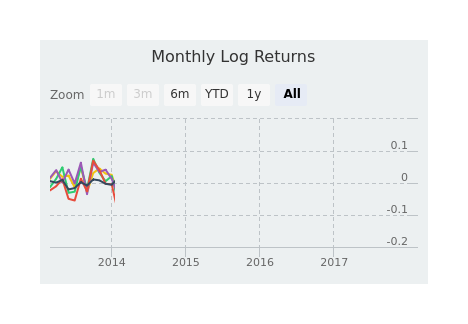
\includegraphics{bookdown_files/figure-latex/unnamed-chunk-34-1.png}

Take a look at the chart. It has a line for the monthly log returns of
each our ETFs (and in my opinion it's starting to get crowded). Do any
months jump out at us? EEM looks to have suffered at the beginning of
2014

Highcharter also has the capacity for histogram making. One method is to
first call the base function \texttt{hist} on the data along with the
arguments for breaks and \texttt{plot\ =\ FALSE}. Then we can call
\texttt{hchart} on that object.

\begin{Shaded}
\begin{Highlighting}[]
\NormalTok{hc_hist <-}\StringTok{ }\KeywordTok{hist}\NormalTok{(asset_returns_xts[, symbols[}\DecValTok{1}\NormalTok{]], }\DataTypeTok{breaks =} \DecValTok{50}\NormalTok{, }\DataTypeTok{plot =} \OtherTok{FALSE}\NormalTok{)}

\KeywordTok{hchart}\NormalTok{(hc_hist) }\OperatorTok\StringTok{ }
\StringTok{  }\KeywordTok{hc_title}\NormalTok{(}\DataTypeTok{text =} \KeywordTok{paste}\NormalTok{(symbols[}\DecValTok{1}\NormalTok{], }\StringTok{"Log Returns Distribution"}\NormalTok{, }\DataTypeTok{sep =} \StringTok{" "}\NormalTok{))}
\end{Highlighting}
\end{Shaded}

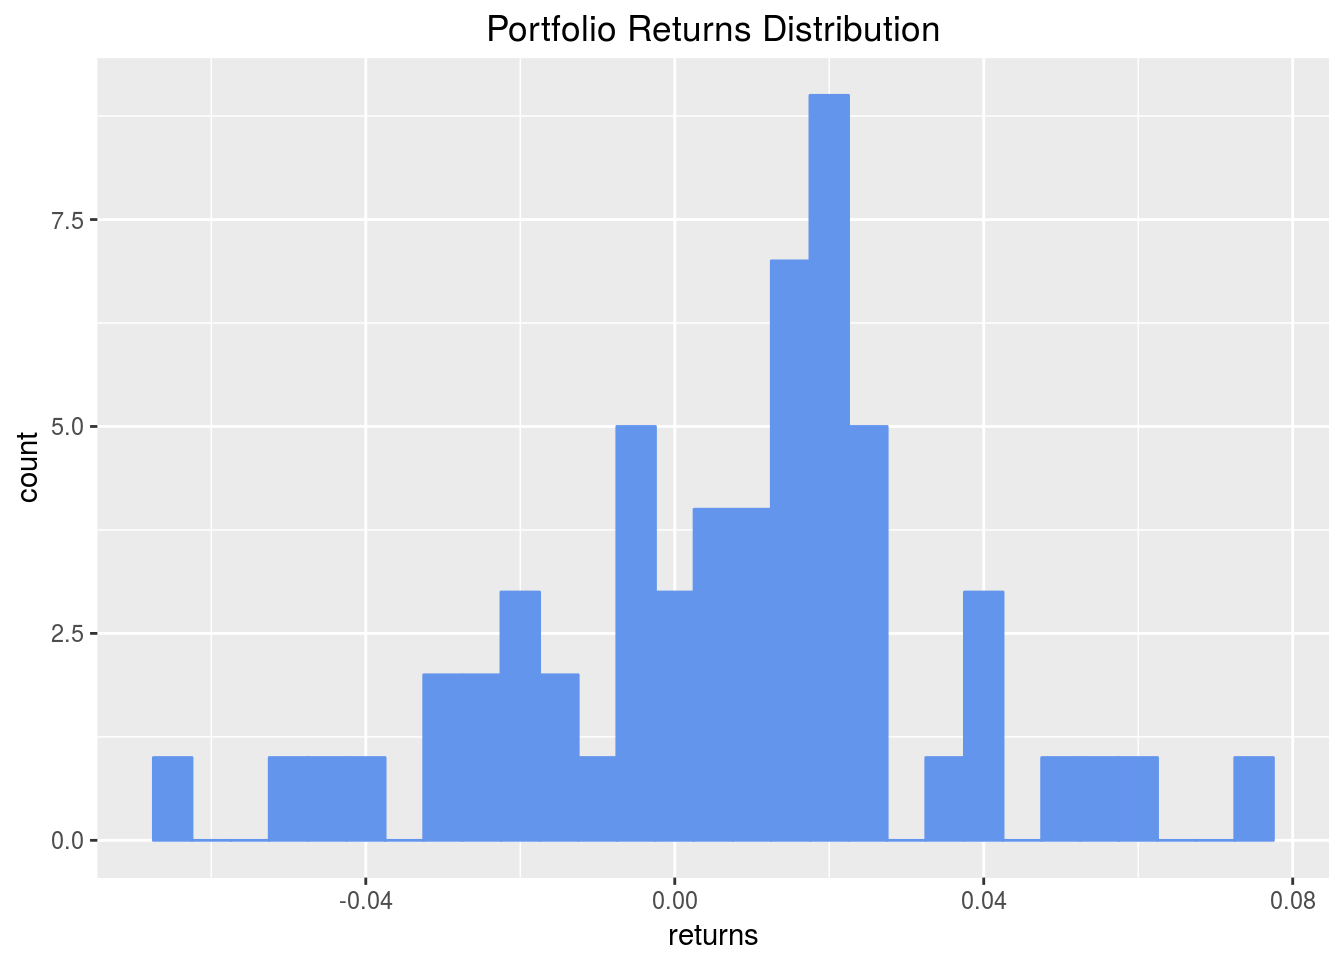
\includegraphics{bookdown_files/figure-latex/unnamed-chunk-35-1.png}

That's a nice histogram but \texttt{highcharter} doesn't have a smooth
way to create 5 histograms as we need to do.

Luckily, we can the \texttt{ggplot2} package from the tidyverse and we
will operat on our tidy data frame \texttt{assets\_returns\_long}.

We call
\texttt{ggplot(aes(x\ =\ returns,\ fill\ =\ asset))\ +\ geom\_histogram(alpha\ =\ 0.25,\ binwidth\ =\ .005)}
and because the data frame is grouped by the `asset' column,
\texttt{ggplot()} knows to chart a separate histogram for each asset.
\texttt{ggplot()} will automatically include a legend since we included
\texttt{fill\ =\ asset} in the \texttt{aes()} call.

\begin{Shaded}
\begin{Highlighting}[]
\KeywordTok{theme_update}\NormalTok{(}\DataTypeTok{plot.title =} \KeywordTok{element_text}\NormalTok{(}\DataTypeTok{hjust =} \FloatTok{0.5}\NormalTok{))}

\NormalTok{asset_returns_long }\OperatorTok\StringTok{ }
\StringTok{  }\KeywordTok{ggplot}\NormalTok{(}\KeywordTok{aes}\NormalTok{(}\DataTypeTok{x =}\NormalTok{ returns, }\DataTypeTok{fill =}\NormalTok{ asset)) }\OperatorTok{+}\StringTok{ }
\StringTok{  }\KeywordTok{geom_histogram}\NormalTok{(}\DataTypeTok{alpha =} \FloatTok{0.25}\NormalTok{, }\DataTypeTok{binwidth =}\NormalTok{ .}\DecValTok{005}\NormalTok{)}
\end{Highlighting}
\end{Shaded}

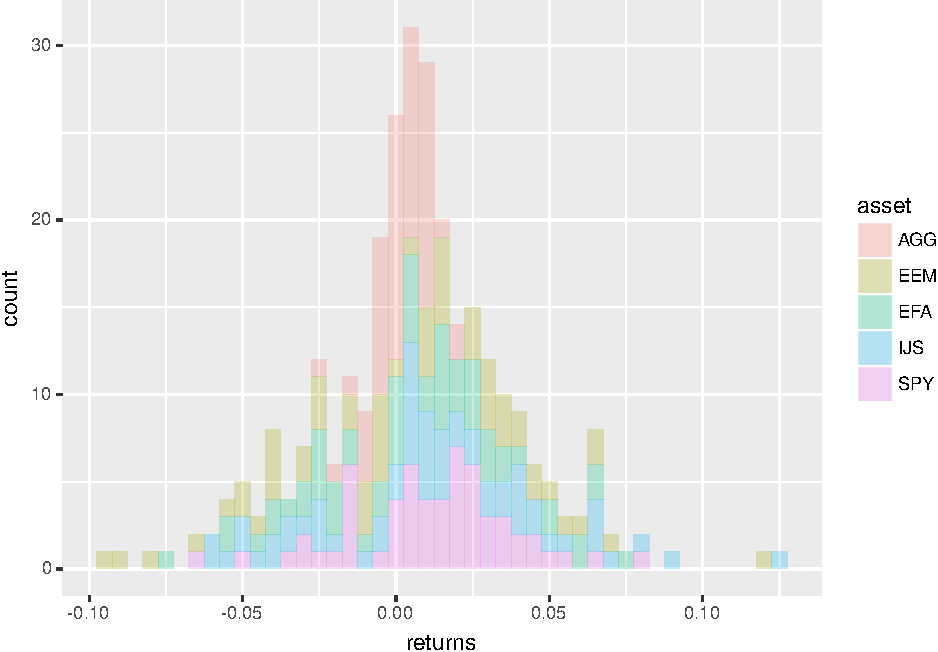
\includegraphics{bookdown_files/figure-latex/unnamed-chunk-36-1.pdf}
That looks nice, but it would be convenient to separate by asset. Let's
use \texttt{facet\_wrap(\textasciitilde{}asset)} to break into 5
separate chars and add a title with \texttt{ggtitle}.

\begin{Shaded}
\begin{Highlighting}[]
\NormalTok{asset_returns_long }\OperatorTok\StringTok{ }
\StringTok{  }\KeywordTok{ggplot}\NormalTok{(}\KeywordTok{aes}\NormalTok{(}\DataTypeTok{x =}\NormalTok{ returns, }\DataTypeTok{fill =}\NormalTok{ asset)) }\OperatorTok{+}\StringTok{ }
\StringTok{  }\KeywordTok{geom_histogram}\NormalTok{(}\DataTypeTok{alpha =} \FloatTok{0.25}\NormalTok{, }\DataTypeTok{binwidth =}\NormalTok{ .}\DecValTok{01}\NormalTok{) }\OperatorTok{+}\StringTok{ }
\StringTok{  }\KeywordTok{facet_wrap}\NormalTok{(}\OperatorTok{~}\NormalTok{asset) }\OperatorTok{+}\StringTok{ }
\StringTok{  }\KeywordTok{ggtitle}\NormalTok{(}\StringTok{"Monthly Returns Since 2013"}\NormalTok{)}
\end{Highlighting}
\end{Shaded}

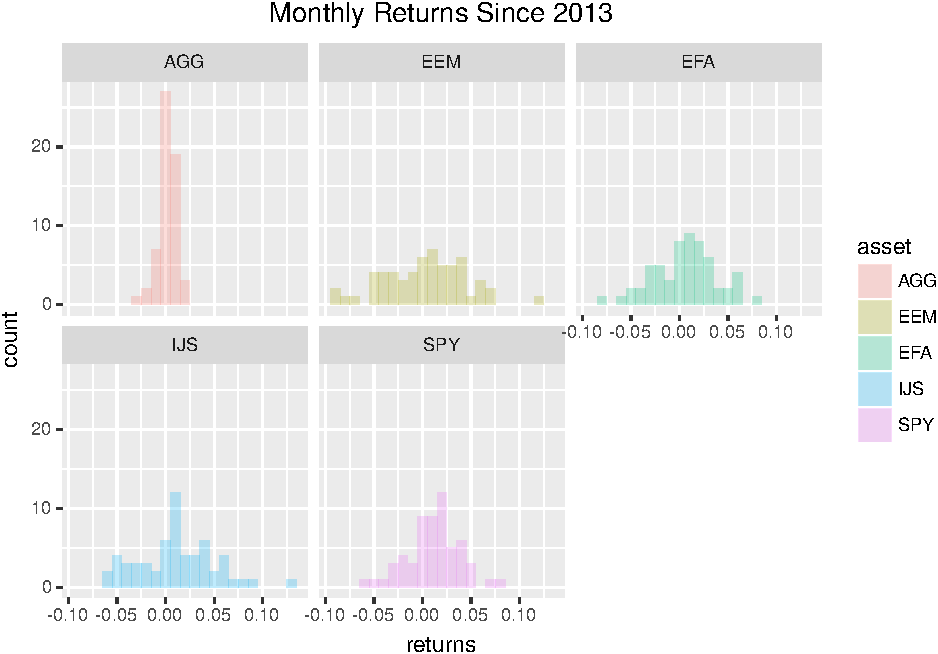
\includegraphics{bookdown_files/figure-latex/unnamed-chunk-37-1.pdf}

Maybe we prefer to use a density line to visualize the various
distributions. We can use the
\texttt{stat\_density(geom\ =\ "line",\ alpha\ =\ 1)} function to do
this. The \texttt{alpha} argument is selecting a line thickness. Let's
also add a label to the x and y axis with the \texttt{xlab} and
\texttt{ylab} functions.

\begin{Shaded}
\begin{Highlighting}[]
\NormalTok{asset_returns_long }\OperatorTok\StringTok{ }
\StringTok{  }\KeywordTok{ggplot}\NormalTok{(}\KeywordTok{aes}\NormalTok{(}\DataTypeTok{x =}\NormalTok{ returns, }\DataTypeTok{colour =}\NormalTok{ asset, }\DataTypeTok{fill =}\NormalTok{ asset)) }\OperatorTok{+}
\StringTok{  }\KeywordTok{stat_density}\NormalTok{(}\DataTypeTok{geom =} \StringTok{"line"}\NormalTok{, }\DataTypeTok{alpha =} \DecValTok{1}\NormalTok{) }\OperatorTok{+}
\StringTok{  }\KeywordTok{ggtitle}\NormalTok{(}\StringTok{"Monthly Returns Since 2005"}\NormalTok{) }\OperatorTok{+}
\StringTok{  }\KeywordTok{xlab}\NormalTok{(}\StringTok{"monthly returns"}\NormalTok{) }\OperatorTok{+}
\StringTok{  }\KeywordTok{ylab}\NormalTok{(}\StringTok{"distribution"}\NormalTok{) }
\end{Highlighting}
\end{Shaded}

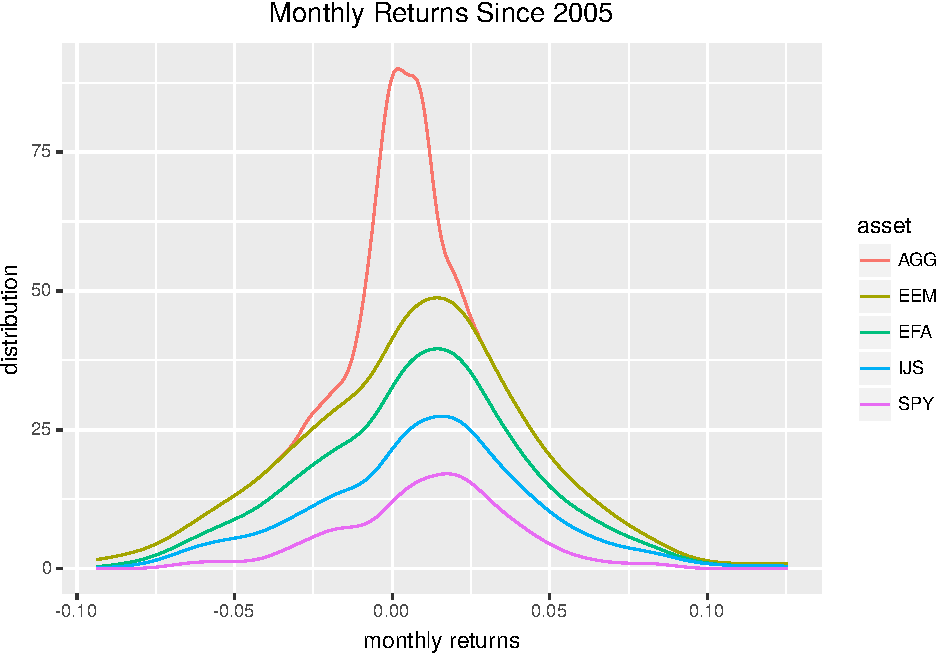
\includegraphics{bookdown_files/figure-latex/unnamed-chunk-38-1.pdf}

That chart is quite digestible, but we can also
\texttt{facet\_wrap(\textasciitilde{}asset)} to break the densities out
into individual charts.

\begin{Shaded}
\begin{Highlighting}[]
\NormalTok{asset_returns_long }\OperatorTok\StringTok{ }
\StringTok{  }\KeywordTok{ggplot}\NormalTok{(}\KeywordTok{aes}\NormalTok{(}\DataTypeTok{x =}\NormalTok{ returns, }\DataTypeTok{colour =}\NormalTok{ asset, }\DataTypeTok{fill =}\NormalTok{ asset)) }\OperatorTok{+}
\StringTok{  }\KeywordTok{stat_density}\NormalTok{(}\DataTypeTok{geom =} \StringTok{"line"}\NormalTok{, }\DataTypeTok{alpha =} \DecValTok{1}\NormalTok{) }\OperatorTok{+}
\StringTok{  }\KeywordTok{facet_wrap}\NormalTok{(}\OperatorTok{~}\NormalTok{asset) }\OperatorTok{+}
\StringTok{  }\KeywordTok{ggtitle}\NormalTok{(}\StringTok{"Monthly Returns Since 2005"}\NormalTok{) }\OperatorTok{+}
\StringTok{  }\KeywordTok{xlab}\NormalTok{(}\StringTok{"monthly returns"}\NormalTok{) }\OperatorTok{+}
\StringTok{  }\KeywordTok{ylab}\NormalTok{(}\StringTok{"distribution"}\NormalTok{) }
\end{Highlighting}
\end{Shaded}

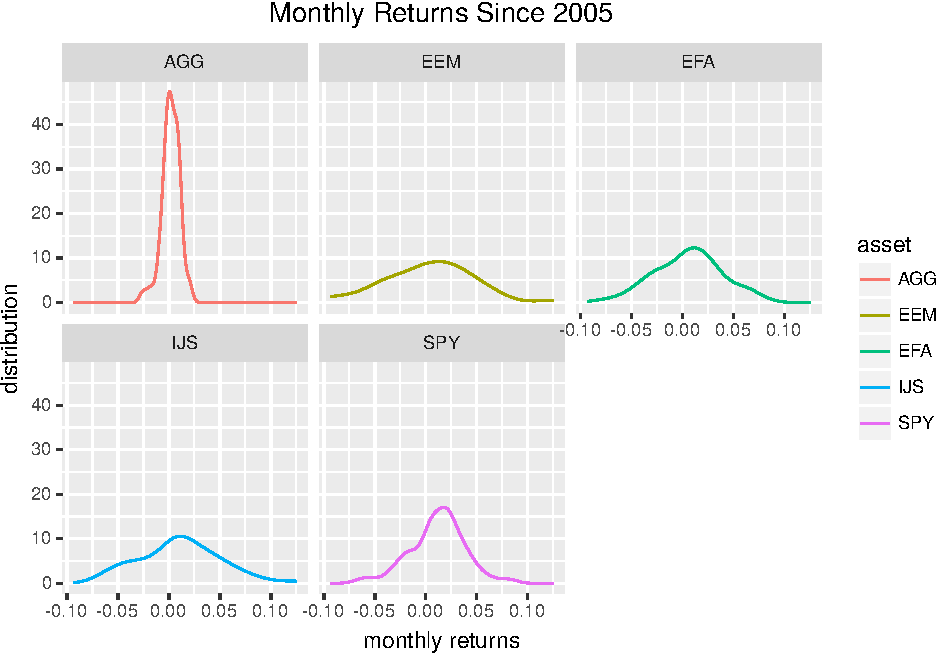
\includegraphics{bookdown_files/figure-latex/unnamed-chunk-39-1.pdf}

Okay, we have made histograms and density plots. Perhaps we would like
to combine both of those into one chart. \texttt{ggplot()} works in
aesthetic layers, which means we can chart a historgram in one layer,
and then add a layer with a density chart.

\begin{Shaded}
\begin{Highlighting}[]
\NormalTok{asset_returns_long }\OperatorTok\StringTok{ }
\StringTok{  }\KeywordTok{ggplot}\NormalTok{(}\KeywordTok{aes}\NormalTok{(}\DataTypeTok{x =}\NormalTok{ returns, }\DataTypeTok{colour =}\NormalTok{ asset, }\DataTypeTok{fill =}\NormalTok{ asset)) }\OperatorTok{+}
\StringTok{  }\KeywordTok{stat_density}\NormalTok{(}\DataTypeTok{geom =} \StringTok{"line"}\NormalTok{, }\DataTypeTok{alpha =} \DecValTok{1}\NormalTok{) }\OperatorTok{+}
\StringTok{  }\KeywordTok{geom_histogram}\NormalTok{(}\DataTypeTok{alpha =} \FloatTok{0.25}\NormalTok{, }\DataTypeTok{binwidth =}\NormalTok{ .}\DecValTok{01}\NormalTok{) }\OperatorTok{+}
\StringTok{  }\KeywordTok{facet_wrap}\NormalTok{(}\OperatorTok{~}\NormalTok{asset) }\OperatorTok{+}
\StringTok{  }\KeywordTok{ggtitle}\NormalTok{(}\StringTok{"Monthly Returns Since 2005"}\NormalTok{) }\OperatorTok{+}
\StringTok{  }\KeywordTok{xlab}\NormalTok{(}\StringTok{"monthly returns"}\NormalTok{) }\OperatorTok{+}
\StringTok{  }\KeywordTok{ylab}\NormalTok{(}\StringTok{"distribution"}\NormalTok{)}
\end{Highlighting}
\end{Shaded}

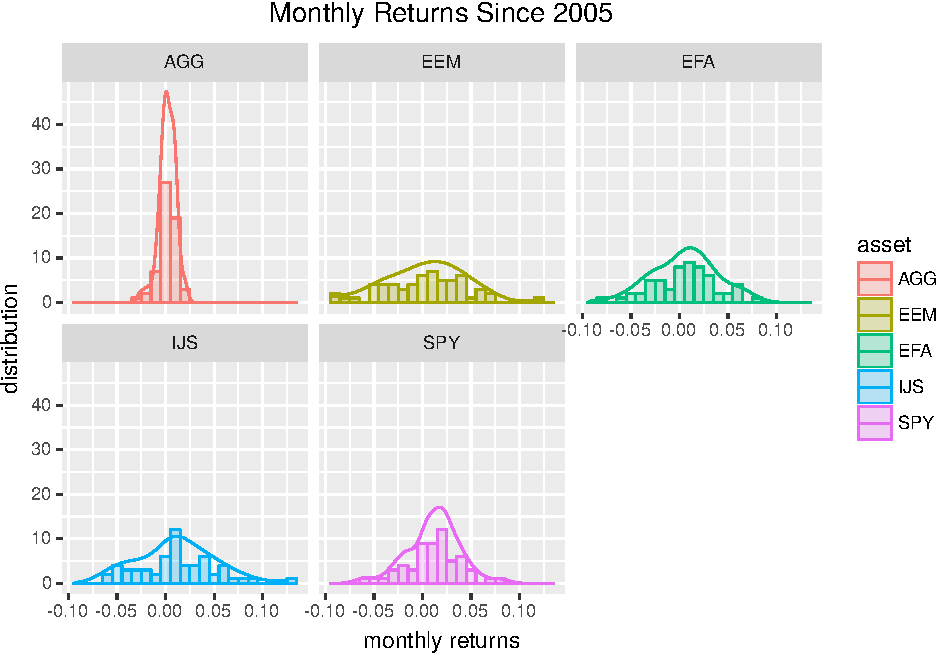
\includegraphics{bookdown_files/figure-latex/unnamed-chunk-40-1.pdf}

We now have one chart, with histograms and line densities broken out for
each of our assets. This would scale nicely if we had more assets and
wanted to peek at more distributions of returns.

\chapter{From Individual Assets to Portfolio
Returns}\label{from-individual-assets-to-portfolio-returns}

\subsection*{Visualize this stuff}\label{visualize-this-stuff}


\chapter{Growth of a Dollar}\label{growth-of-a-dollar}

\subsection*{Visualize this stuff}\label{visualize-this-stuff-1}


\chapter{Risk}\label{risk}

Let's check out a Shiny app.

\begin{figure}
\centering
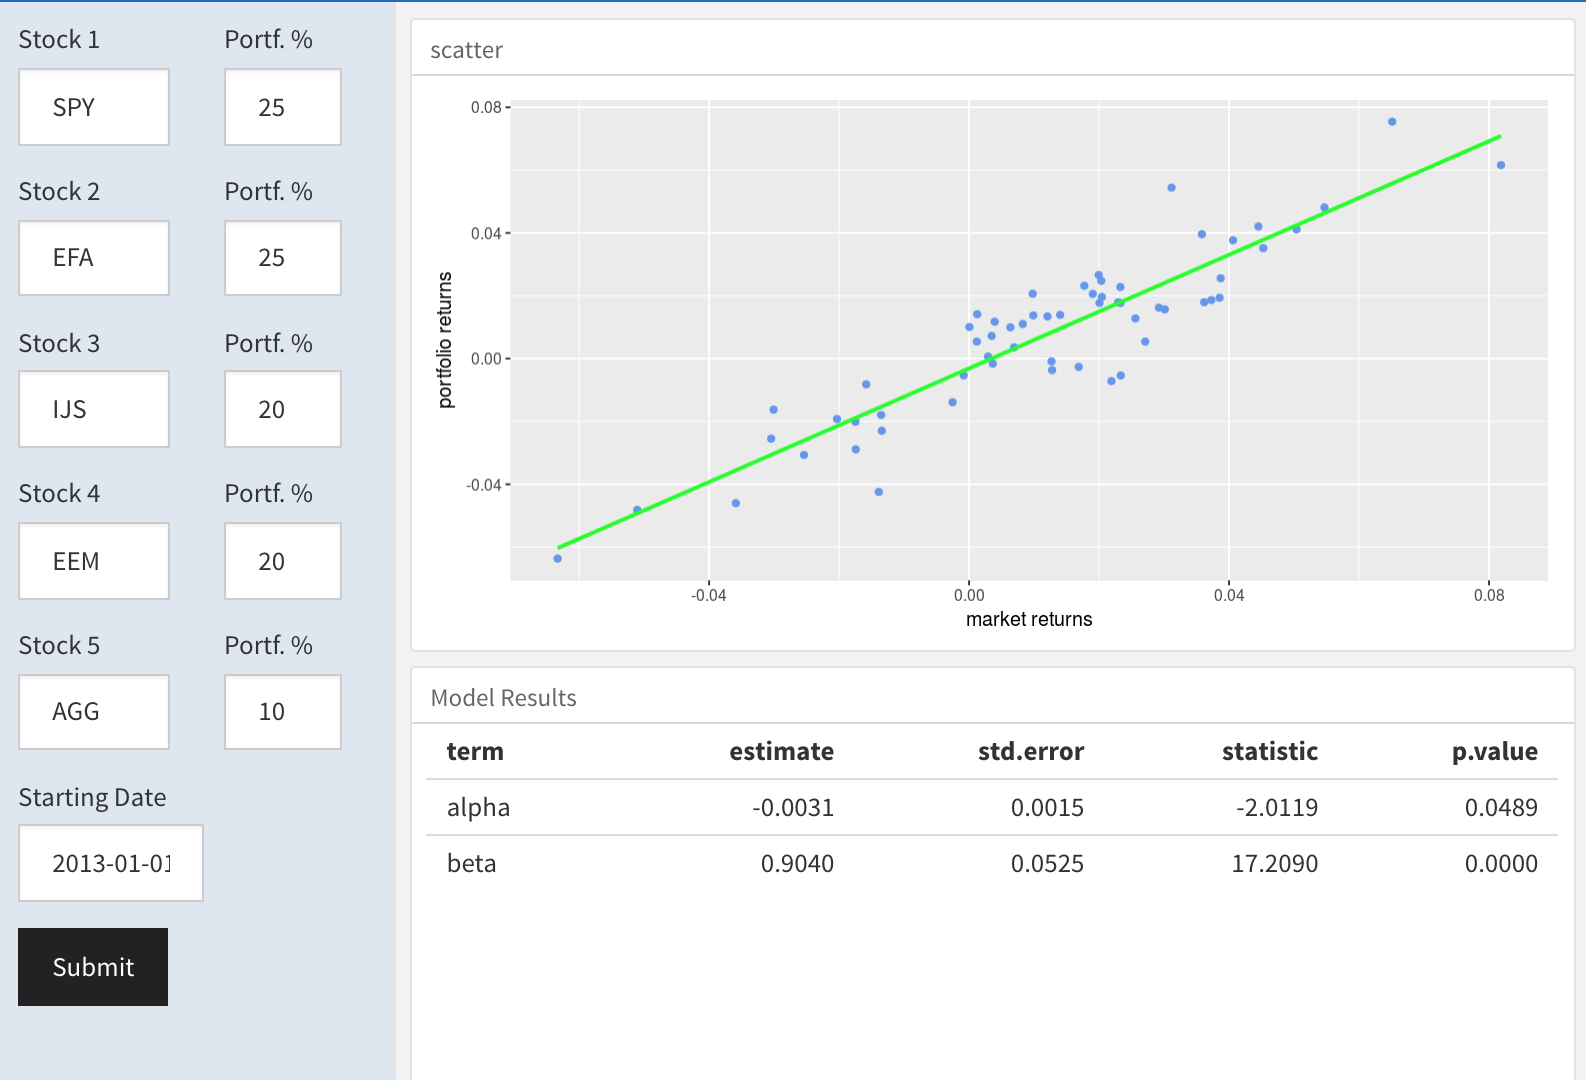
\includegraphics{snapshots/snapshot-test.png}
\caption{CAPM Beta Shiny App}
\end{figure}

\begin{figure}
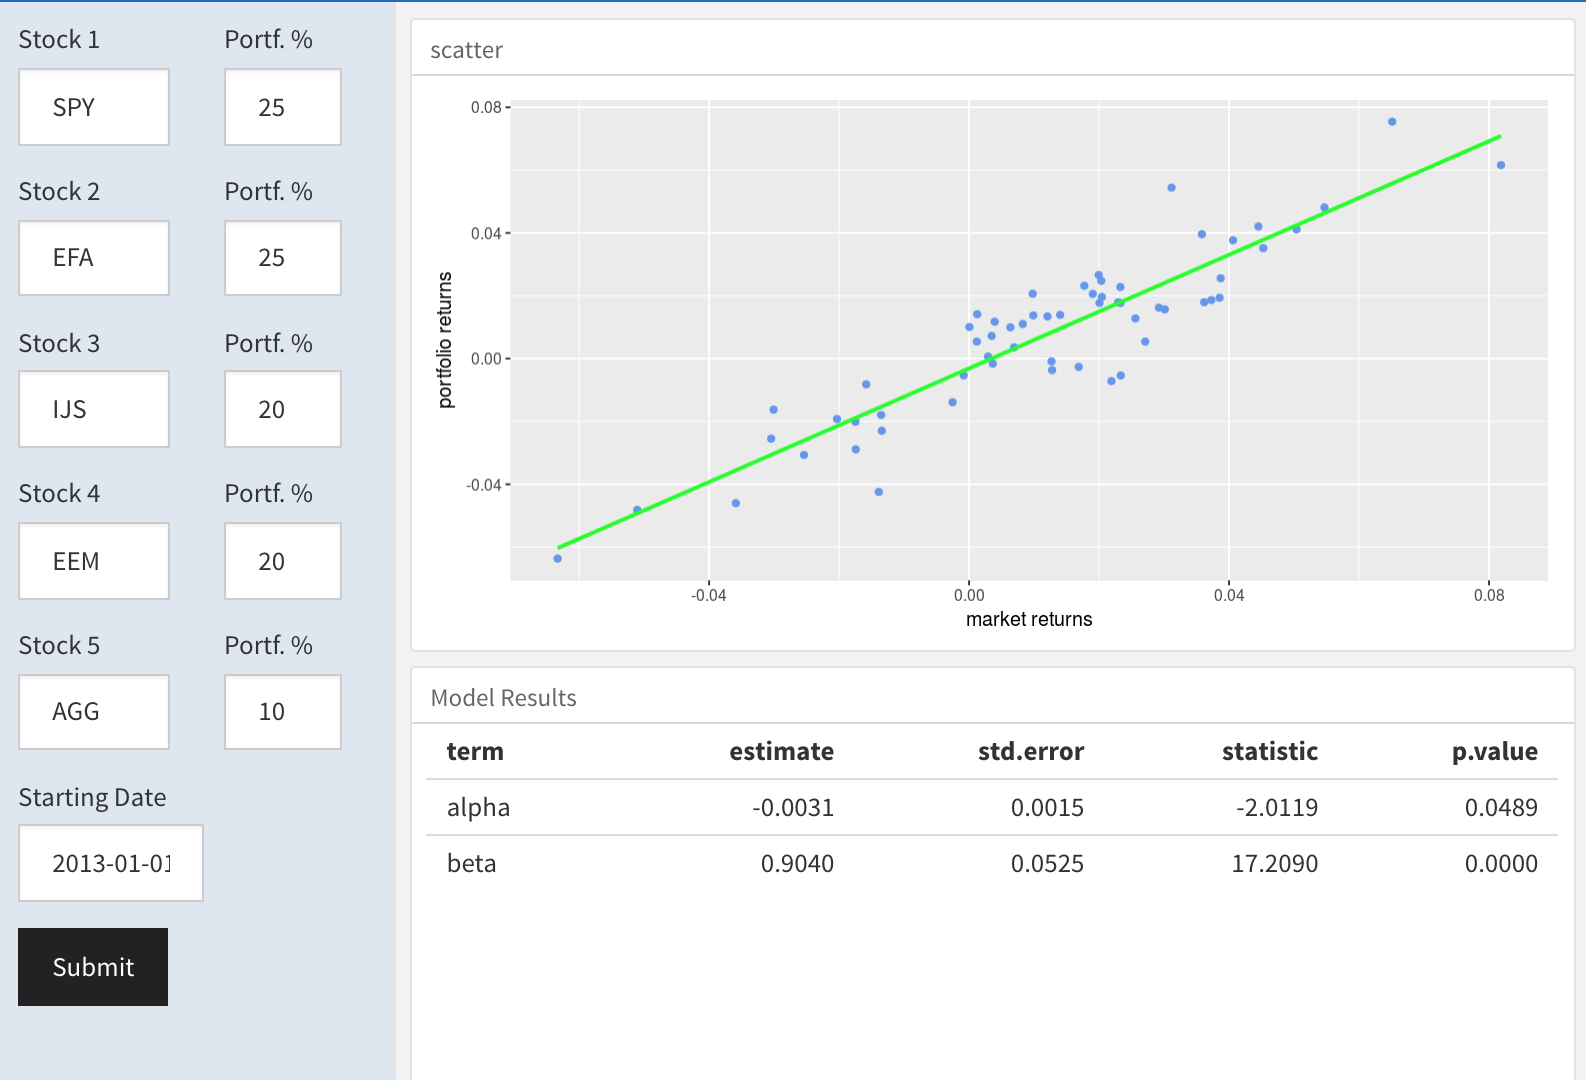
\includegraphics[width=1\linewidth]{snapshots/capm-beta-shiny} \caption{CAPM Beta Shiny App}\label{fig:unnamed-chunk-41}
\end{figure}

\chapter{Portfolio Theory}\label{portfolio-theory}

Jonathan Regenstein is the Director of Financial Services practice at
RStudio.

\begin{figure}
\centering
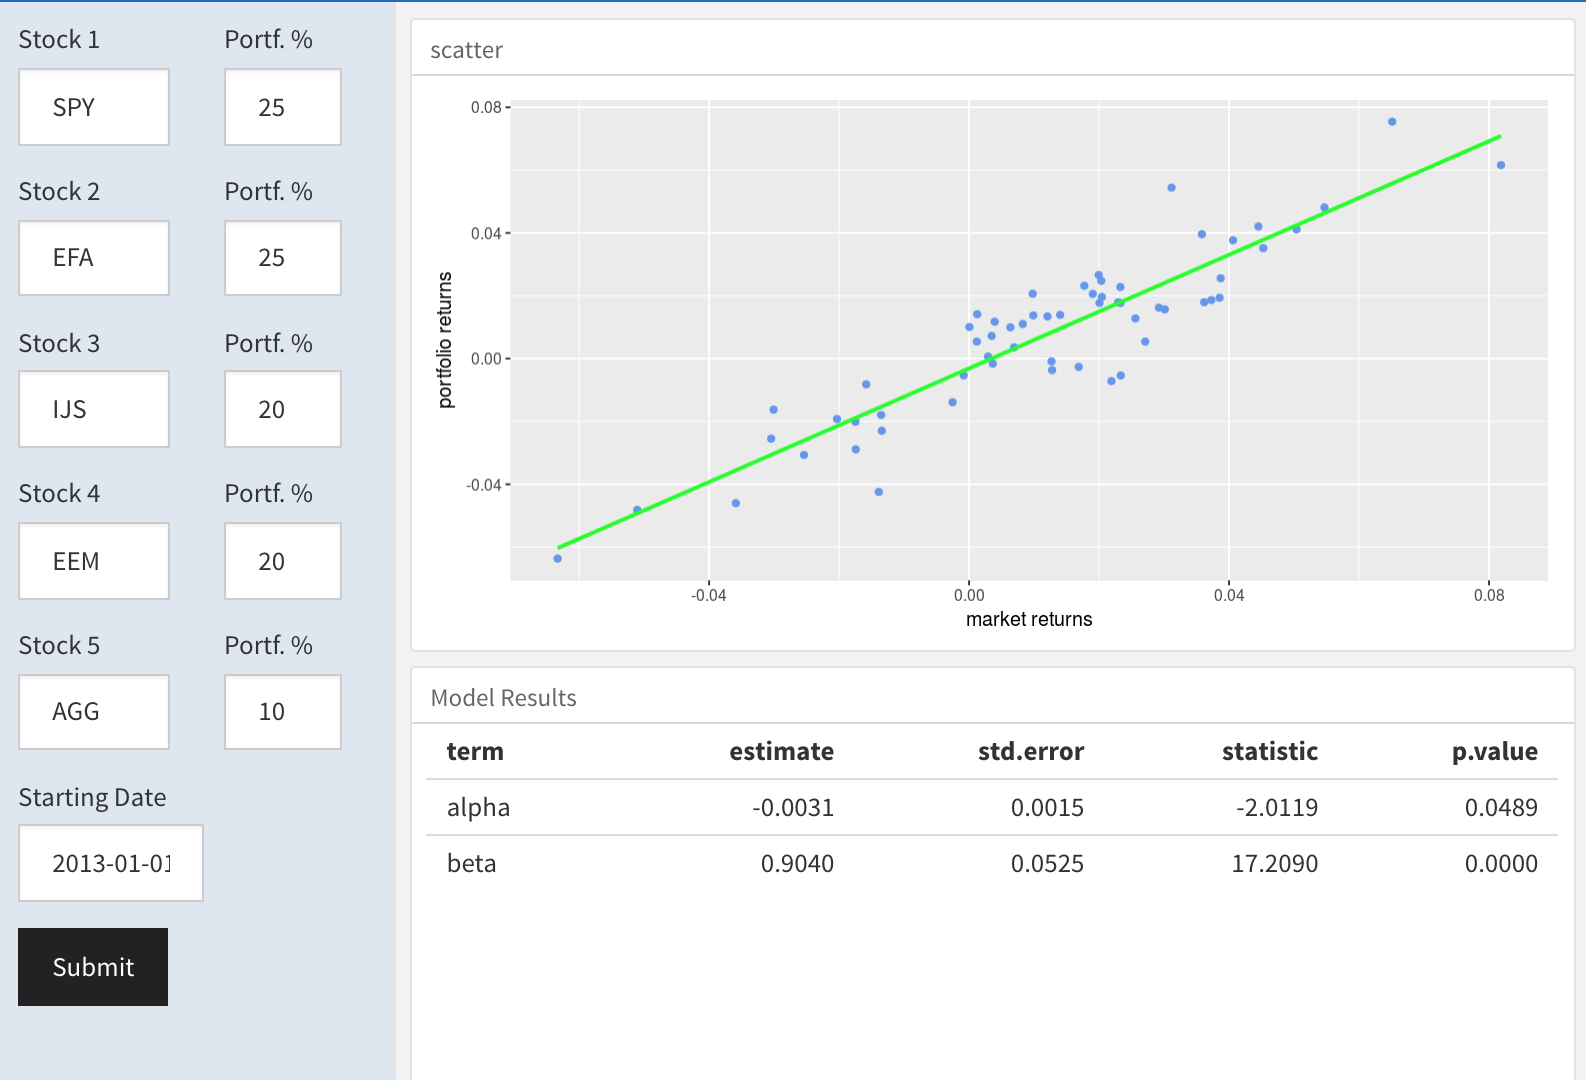
\includegraphics{snapshots/capm-beta-shiny.png}
\caption{Capm Beta Shiny}
\end{figure}

\begin{figure}
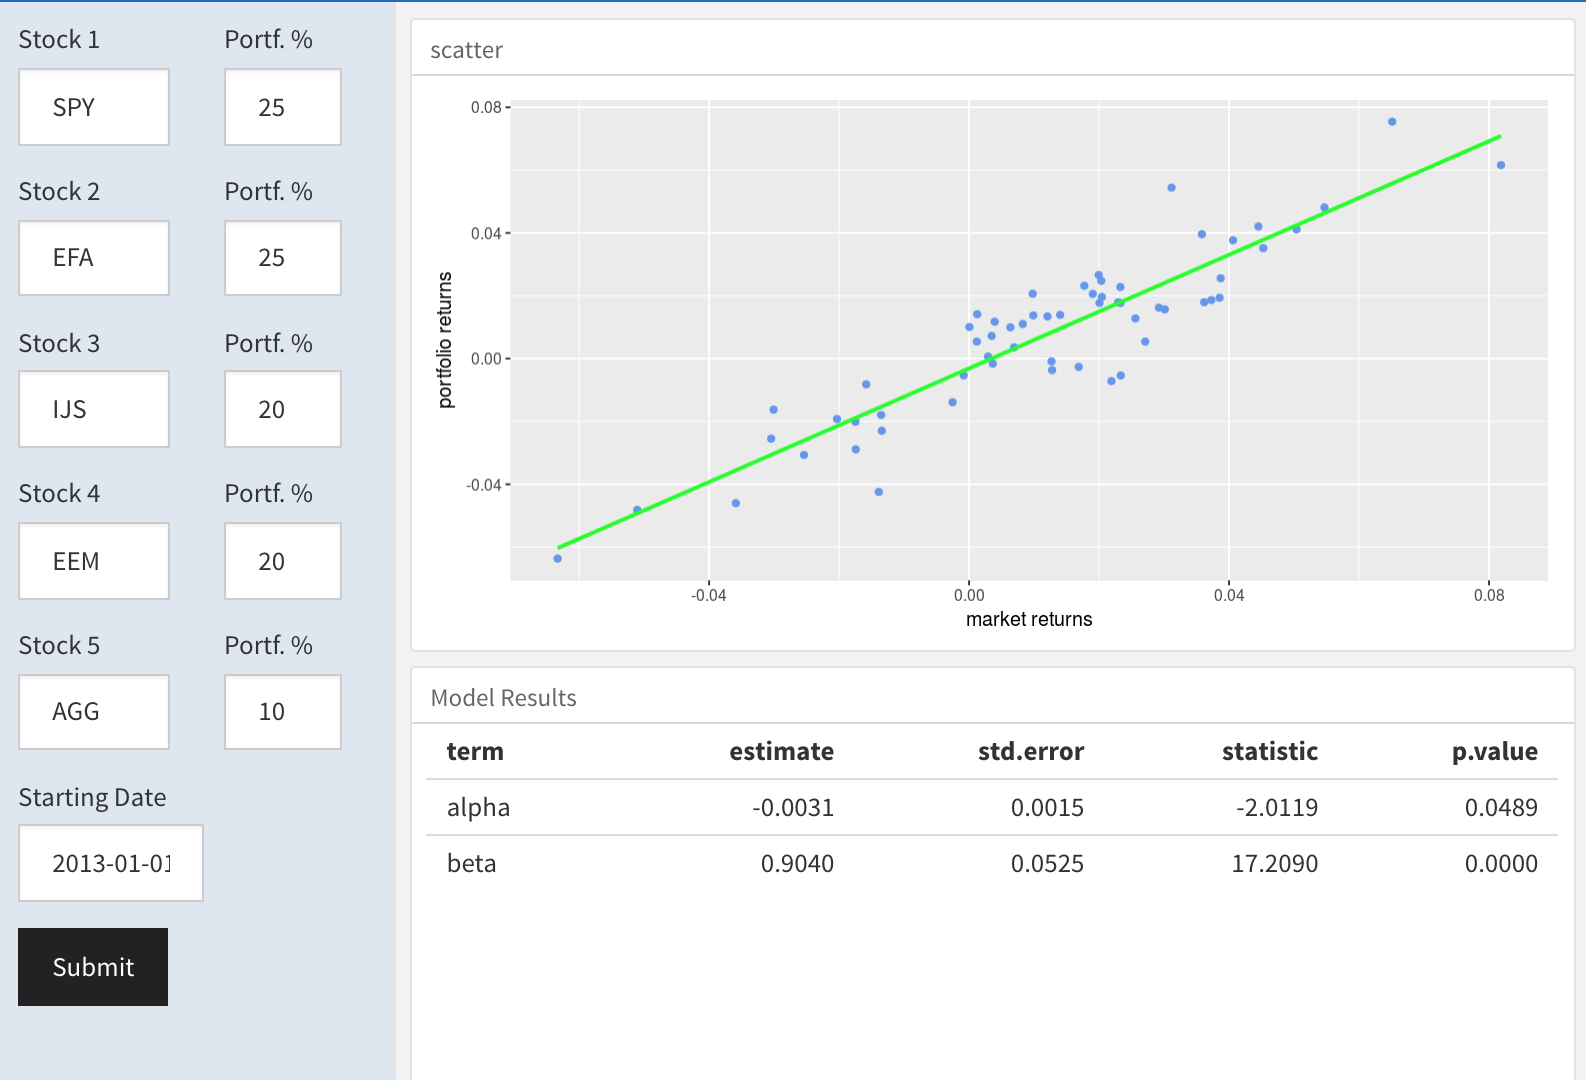
\includegraphics[width=1\linewidth]{snapshots/capm-beta-shiny.png} \caption{Capm Beta Shiny}\label{fig:unnamed-chunk-42}
\end{figure}

\chapter{montecarlo}\label{montecarlo}

\cleardoublepage 

\appendix \addcontentsline{toc}{chapter}{\appendixname}


\chapter{More to Say}\label{more-to-say}

Yeah! I have finished my book, but I have more to say about some topics.
Let me explain them in this appendix.

To know more about \textbf{bookdown}, see \url{https://bookdown.org}.

\chapter*{Appendix 2}\label{appendix-2}


\chapter{Returns Source File}\label{returns-source-file}

\begin{Shaded}
\begin{Highlighting}[]
\KeywordTok{library}\NormalTok{(tidyverse)}
\KeywordTok{library}\NormalTok{(tidyquant)}
\KeywordTok{library}\NormalTok{(timetk)}
\KeywordTok{library}\NormalTok{(tibbletime)}
\end{Highlighting}
\end{Shaded}

\begin{Shaded}
\begin{Highlighting}[]
\CommentTok{# The symbols vector holds our tickers. }
\NormalTok{symbols <-}\StringTok{ }\KeywordTok{c}\NormalTok{(}\StringTok{"SPY"}\NormalTok{,}\StringTok{"EFA"}\NormalTok{, }\StringTok{"IJS"}\NormalTok{, }\StringTok{"EEM"}\NormalTok{,}\StringTok{"AGG"}\NormalTok{)}

\CommentTok{# The prices object will hold our raw price data throughout this book.}
\NormalTok{prices <-}\StringTok{ }
\StringTok{  }\KeywordTok{getSymbols}\NormalTok{(symbols, }\DataTypeTok{src =} \StringTok{'yahoo'}\NormalTok{, }\DataTypeTok{from =} \StringTok{"2013-01-01"}\NormalTok{, }\DataTypeTok{to =} \StringTok{"2017-12-31"}\NormalTok{, }
             \DataTypeTok{auto.assign =} \OtherTok{TRUE}\NormalTok{, }\DataTypeTok{warnings =} \OtherTok{FALSE}\NormalTok{) }\OperatorTok\StringTok{ }
\StringTok{  }\KeywordTok{map}\NormalTok{(}\OperatorTok{~}\KeywordTok{Ad}\NormalTok{(}\KeywordTok{get}\NormalTok{(.))) }\OperatorTok\StringTok{ }
\StringTok{  }\KeywordTok{reduce}\NormalTok{(merge) }\OperatorTok
\StringTok{  `}\DataTypeTok{colnames<-}\StringTok{`}\NormalTok{(symbols)}
\end{Highlighting}
\end{Shaded}

\begin{Shaded}
\begin{Highlighting}[]
\NormalTok{prices_monthly <-}\StringTok{ }\KeywordTok{to.monthly}\NormalTok{(prices, }\DataTypeTok{indexAt =} \StringTok{"last"}\NormalTok{, }\DataTypeTok{OHLC =} \OtherTok{FALSE}\NormalTok{)}

\NormalTok{asset_returns_xts <-}\StringTok{ }\KeywordTok{na.omit}\NormalTok{(}\KeywordTok{Return.calculate}\NormalTok{(prices_monthly, }\DataTypeTok{method =} \StringTok{"log"}\NormalTok{))}
\end{Highlighting}
\end{Shaded}

\begin{Shaded}
\begin{Highlighting}[]
\NormalTok{asset_returns_dplyr_byhand <-}\StringTok{ }
\StringTok{  }\NormalTok{prices }\OperatorTok\StringTok{ }
\StringTok{  }\KeywordTok{to.monthly}\NormalTok{(}\DataTypeTok{indexAt =} \StringTok{"lastof"}\NormalTok{, }\DataTypeTok{OHLC =} \OtherTok{FALSE}\NormalTok{) }\OperatorTok\StringTok{ }
\StringTok{  }\KeywordTok{tk_tbl}\NormalTok{(}\DataTypeTok{preserve_index =} \OtherTok{TRUE}\NormalTok{, }\DataTypeTok{rename_index =} \StringTok{"date"}\NormalTok{) }\OperatorTok
\StringTok{  }\KeywordTok{gather}\NormalTok{(asset, returns, }\OperatorTok{-}\NormalTok{date) }\OperatorTok\StringTok{ }
\StringTok{  }\KeywordTok{group_by}\NormalTok{(asset) }\OperatorTok\StringTok{  }
\StringTok{  }\KeywordTok{mutate}\NormalTok{(}\DataTypeTok{returns =}\NormalTok{ (}\KeywordTok{log}\NormalTok{(returns) }\OperatorTok{-}\StringTok{ }\KeywordTok{log}\NormalTok{(}\KeywordTok{lag}\NormalTok{(returns)))) }\OperatorTok
\StringTok{  }\KeywordTok{spread}\NormalTok{(asset, returns) }\OperatorTok\StringTok{ }
\StringTok{  }\KeywordTok{select}\NormalTok{(date, symbols) }\OperatorTok\StringTok{ }
\StringTok{  }\KeywordTok{slice}\NormalTok{(}\OperatorTok{-}\DecValTok{1}\NormalTok{)}
\end{Highlighting}
\end{Shaded}

\begin{Shaded}
\begin{Highlighting}[]
\NormalTok{asset_returns_tq_builtin <-}\StringTok{ }\NormalTok{prices }\OperatorTok
\StringTok{  }\KeywordTok{tk_tbl}\NormalTok{(}\DataTypeTok{preserve_index =} \OtherTok{TRUE}\NormalTok{, }\DataTypeTok{rename_index =} \StringTok{"date"}\NormalTok{) }\OperatorTok
\StringTok{  }\KeywordTok{gather}\NormalTok{(asset, prices, }\OperatorTok{-}\NormalTok{date) }\OperatorTok\StringTok{ }
\StringTok{  }\KeywordTok{group_by}\NormalTok{(asset) }\OperatorTok
\StringTok{  }\KeywordTok{tq_transmute}\NormalTok{(}\DataTypeTok{mutate_fun =}\NormalTok{ periodReturn, }\DataTypeTok{period =} \StringTok{"monthly"}\NormalTok{, }\DataTypeTok{type =} \StringTok{"log"}\NormalTok{) }\OperatorTok\StringTok{ }
\StringTok{  }\KeywordTok{spread}\NormalTok{(asset, monthly.returns) }\OperatorTok\StringTok{ }
\StringTok{  }\KeywordTok{select}\NormalTok{(date, symbols) }\OperatorTok\StringTok{ }
\StringTok{  }\KeywordTok{slice}\NormalTok{(}\OperatorTok{-}\DecValTok{1}\NormalTok{)}
\end{Highlighting}
\end{Shaded}

\begin{Shaded}
\begin{Highlighting}[]
\NormalTok{asset_returns_tbltime <-}\StringTok{ }
\StringTok{  }\NormalTok{prices }\OperatorTok\StringTok{ }
\StringTok{  }\KeywordTok{to.monthly}\NormalTok{(}\DataTypeTok{indexAt =} \StringTok{"lastof"}\NormalTok{, }\DataTypeTok{OHLC =} \OtherTok{FALSE}\NormalTok{) }\OperatorTok
\StringTok{  }\KeywordTok{tk_tbl}\NormalTok{(}\DataTypeTok{preserve_index =} \OtherTok{TRUE}\NormalTok{, }\DataTypeTok{rename_index =} \StringTok{"date"}\NormalTok{) }\OperatorTok
\StringTok{  }\KeywordTok{tbl_time}\NormalTok{(}\DataTypeTok{index =} \StringTok{"date"}\NormalTok{) }\OperatorTok\StringTok{ }
\StringTok{  }\KeywordTok{gather}\NormalTok{(asset, returns, }\OperatorTok{-}\NormalTok{date) }\OperatorTok\StringTok{ }
\StringTok{  }\KeywordTok{group_by}\NormalTok{(asset) }\OperatorTok\StringTok{ }
\StringTok{  }\KeywordTok{tq_transmute}\NormalTok{(}\DataTypeTok{mutate_fun =}\NormalTok{ periodReturn, }\DataTypeTok{type =} \StringTok{"log"}\NormalTok{) }\OperatorTok\StringTok{ }
\StringTok{  }\KeywordTok{spread}\NormalTok{(asset, monthly.returns) }\OperatorTok\StringTok{ }
\StringTok{  }\KeywordTok{select}\NormalTok{(date, symbols) }\OperatorTok\StringTok{ }
\StringTok{  }\KeywordTok{slice}\NormalTok{(}\OperatorTok{-}\DecValTok{1}\NormalTok{)}
\end{Highlighting}
\end{Shaded}

\begin{Shaded}
\begin{Highlighting}[]
\NormalTok{asset_returns_long <-}\StringTok{ }
\StringTok{  }\NormalTok{asset_returns_dplyr_byhand }\OperatorTok\StringTok{ }
\StringTok{  }\KeywordTok{gather}\NormalTok{(asset, returns, }\OperatorTok{-}\NormalTok{date)}
\end{Highlighting}
\end{Shaded}

\begin{Shaded}
\begin{Highlighting}[]
\NormalTok{w <-}\StringTok{ }\KeywordTok{c}\NormalTok{(}\FloatTok{0.25}\NormalTok{, }\FloatTok{0.25}\NormalTok{, }\FloatTok{0.20}\NormalTok{, }\FloatTok{0.20}\NormalTok{, }\FloatTok{0.10}\NormalTok{)}
\end{Highlighting}
\end{Shaded}

\begin{Shaded}
\begin{Highlighting}[]
\NormalTok{w_}\DecValTok{1}\NormalTok{ <-}\StringTok{ }\NormalTok{w[}\DecValTok{1}\NormalTok{]}
\NormalTok{w_}\DecValTok{2}\NormalTok{ <-}\StringTok{ }\NormalTok{w[}\DecValTok{2}\NormalTok{]}
\NormalTok{w_}\DecValTok{3}\NormalTok{ <-}\StringTok{ }\NormalTok{w[}\DecValTok{3}\NormalTok{]}
\NormalTok{w_}\DecValTok{4}\NormalTok{ <-}\StringTok{ }\NormalTok{w[}\DecValTok{4}\NormalTok{]}
\NormalTok{w_}\DecValTok{5}\NormalTok{ <-}\StringTok{ }\NormalTok{w[}\DecValTok{5}\NormalTok{]}

\NormalTok{asset1 <-}\StringTok{ }\NormalTok{asset_returns_xts[,}\DecValTok{1}\NormalTok{]}
\NormalTok{asset2 <-}\StringTok{ }\NormalTok{asset_returns_xts[,}\DecValTok{2}\NormalTok{]}
\NormalTok{asset3 <-}\StringTok{ }\NormalTok{asset_returns_xts[,}\DecValTok{3}\NormalTok{]}
\NormalTok{asset4 <-}\StringTok{ }\NormalTok{asset_returns_xts[,}\DecValTok{4}\NormalTok{]}
\NormalTok{asset5 <-}\StringTok{ }\NormalTok{asset_returns_xts[,}\DecValTok{5}\NormalTok{]}

\NormalTok{portfolio_returns_byhand <-}\StringTok{   }
\StringTok{  }\NormalTok{(w_}\DecValTok{1} \OperatorTok{*}\StringTok{ }\NormalTok{asset1) }\OperatorTok{+}\StringTok{ }
\StringTok{  }\NormalTok{(w_}\DecValTok{2} \OperatorTok{*}\StringTok{ }\NormalTok{asset2) }\OperatorTok{+}\StringTok{ }
\StringTok{  }\NormalTok{(w_}\DecValTok{3} \OperatorTok{*}\StringTok{ }\NormalTok{asset3) }\OperatorTok{+}
\StringTok{  }\NormalTok{(w_}\DecValTok{4} \OperatorTok{*}\StringTok{ }\NormalTok{asset4) }\OperatorTok{+}\StringTok{ }
\StringTok{  }\NormalTok{(w_}\DecValTok{5} \OperatorTok{*}\StringTok{ }\NormalTok{asset5)}

\KeywordTok{names}\NormalTok{(portfolio_returns_byhand) <-}\StringTok{ "returns"}
\end{Highlighting}
\end{Shaded}

\begin{Shaded}
\begin{Highlighting}[]
\NormalTok{portfolio_returns_xts_rebalanced_monthly <-}\StringTok{ }
\StringTok{  }\KeywordTok{Return.portfolio}\NormalTok{(asset_returns_xts, }\DataTypeTok{weights =}\NormalTok{ w, }\DataTypeTok{rebalance_on =} \StringTok{"months"}\NormalTok{) }\OperatorTok
\StringTok{  `}\DataTypeTok{colnames<-}\StringTok{`}\NormalTok{(}\StringTok{"returns"}\NormalTok{)}

\NormalTok{portfolio_returns_xts_rebalanced_yearly <-}\StringTok{ }
\StringTok{  }\KeywordTok{Return.portfolio}\NormalTok{(asset_returns_xts, }\DataTypeTok{weights =}\NormalTok{ w, }\DataTypeTok{rebalance_on =} \StringTok{"years"}\NormalTok{) }\OperatorTok
\StringTok{  `}\DataTypeTok{colnames<-}\StringTok{`}\NormalTok{(}\StringTok{"returns"}\NormalTok{)}
\end{Highlighting}
\end{Shaded}

\begin{Shaded}
\begin{Highlighting}[]
\NormalTok{portfolio_returns_dplyr_byhand <-}\StringTok{ }
\NormalTok{asset_returns_long }\OperatorTok
\KeywordTok{group_by}\NormalTok{(asset) }\OperatorTok\StringTok{ }
\KeywordTok{mutate}\NormalTok{(}\DataTypeTok{weights =} \KeywordTok{if_else}\NormalTok{(asset }\OperatorTok{==}\StringTok{ }\NormalTok{symbols[}\DecValTok{1}\NormalTok{], w[}\DecValTok{1}\NormalTok{],}
                    \KeywordTok{if_else}\NormalTok{(asset }\OperatorTok{==}\StringTok{ }\NormalTok{symbols[}\DecValTok{2}\NormalTok{], w[}\DecValTok{2}\NormalTok{],}
                        \KeywordTok{if_else}\NormalTok{(asset }\OperatorTok{==}\StringTok{ }\NormalTok{symbols[}\DecValTok{3}\NormalTok{], w[}\DecValTok{3}\NormalTok{],}
                            \KeywordTok{if_else}\NormalTok{(asset }\OperatorTok{==}\StringTok{ }\NormalTok{symbols[}\DecValTok{4}\NormalTok{], w[}\DecValTok{4}\NormalTok{], w[}\DecValTok{5}\NormalTok{])))),}
        \DataTypeTok{weighted_returns =}\NormalTok{ returns }\OperatorTok{*}\StringTok{ }\NormalTok{weights) }\OperatorTok\StringTok{ }
\StringTok{  }\KeywordTok{group_by}\NormalTok{(date) }\OperatorTok\StringTok{ }
\StringTok{  }\KeywordTok{summarise}\NormalTok{(}\DataTypeTok{returns =} \KeywordTok{sum}\NormalTok{(weighted_returns))}
\end{Highlighting}
\end{Shaded}

\begin{Shaded}
\begin{Highlighting}[]
\NormalTok{portfolio_returns_tq_rebalanced_monthly <-}\StringTok{ }
\StringTok{  }\NormalTok{asset_returns_long }\OperatorTok
\StringTok{  }\KeywordTok{tq_portfolio}\NormalTok{(}\DataTypeTok{assets_col  =}\NormalTok{ asset, }
               \DataTypeTok{returns_col =}\NormalTok{ returns,}
               \DataTypeTok{weights     =}\NormalTok{ w,}
               \DataTypeTok{col_rename  =} \StringTok{"returns"}\NormalTok{,}
               \DataTypeTok{rebalance_on =} \StringTok{"months"}\NormalTok{)}

\NormalTok{portfolio_returns_tq_rebalanced_yearly <-}\StringTok{ }
\StringTok{  }\NormalTok{asset_returns_long }\OperatorTok
\StringTok{  }\KeywordTok{tq_portfolio}\NormalTok{(}\DataTypeTok{assets_col  =}\NormalTok{ asset, }
               \DataTypeTok{returns_col =}\NormalTok{ returns,}
               \DataTypeTok{weights     =}\NormalTok{ w,}
               \DataTypeTok{col_rename  =} \StringTok{"returns"}\NormalTok{,}
               \DataTypeTok{rebalance_on =} \StringTok{"years"}\NormalTok{)}
\end{Highlighting}
\end{Shaded}

\begin{Shaded}
\begin{Highlighting}[]
\KeywordTok{save}\NormalTok{(}\DataTypeTok{list =} \KeywordTok{ls}\NormalTok{(.GlobalEnv), }\DataTypeTok{file =} \StringTok{"book-data.Rdata"}\NormalTok{)}
\end{Highlighting}
\end{Shaded}

\bibliography{book.bib,packages.bib}

\backmatter
\printindex

\end{document}
